\documentclass[palatino,nochap]{apuntes}

\title{Investigación Operativa}
\author{Víctor de Juan Sanz}
\date{15/16 C2}

\lstset{
    language=R,
    basicstyle=\ttfamily
}


%%%%%%%%%%%%%%%  lstlisting style

\tikzset{point/.style={insert path={ node[scale=2.5*sqrt(\pgflinewidth)]{.} }}}
\usetikzlibrary{calc}
\usepackage{tikztools}
\usepackage{fancysprefs}


\definecolor{codegreen}{rgb}{0,0.6,0}
\definecolor{codegray}{rgb}{0.5,0.5,0.5}
\definecolor{codepurple}{rgb}{0.58,0,0.82}
\definecolor{backcolour}{rgb}{0.95,0.95,0.92}

\lstdefinestyle{mystyle}{
    backgroundcolor=\color{backcolour},
    commentstyle=\color{codegreen},
    keywordstyle=\color{magenta},
    numberstyle=\tiny\color{codegray},
    stringstyle=\color{codepurple},
    basicstyle=\footnotesize,
    breakatwhitespace=false,
    breaklines=true,
    captionpos=b,
    keepspaces=true,
    numbers=left,
    numbersep=5pt,
    showspaces=false,
    showstringspaces=false,
    showtabs=false,
    tabsize=2
}

\usepackage[acronym]{glossaries}        % Glosario/Acrónimos
\makeglossaries
\newacronym{SVM}{SVM}{Support Vector Machine}

\usepackage[most]{tcolorbox}

\tcbset{
    frame code={}
    center title,
    left=0pt,
    right=0pt,
    top=0pt,
    bottom=0pt,
    colback=green!65!blue!80!gray!15!white,
    colframe=white,
    width=\dimexpr\textwidth\relax,
    enlarge left by=0mm,
    boxsep=5pt,
    arc=0pt,outer arc=0pt,
    }

\newcommand{\KKT}[1]{\mbox{KKT}\left(#1\right)}

\newcommand{\goal}[1]{

El \textbf{objetivo} del problema es:  #1}
\newcommand{\restrictions}[6][]{

	Las \textbf{restricciones} del problema son:

	\begin{enumerate}
		\ifthenelse{\equal{#1}{}}{}{\item #1}
		\ifthenelse{\equal{#2}{}}{}{\item #2}
		\ifthenelse{\equal{#3}{}}{}{\item #3}
		\ifthenelse{\equal{#4}{}}{}{\item #4}
		\ifthenelse{\equal{#5}{}}{}{\item #5}
		\ifthenelse{\equal{#6}{}}{}{\item #6}
	\end{enumerate}}



\newenvironment{ioprob}{\begin{tcolorbox}}{\end{tcolorbox}}


% Paquetes adicionales

% --------------------
\usetikzlibrary{patterns}

\begin{document}
\begin{abstract}
Estos son apuntes del curso \textit{Investigación Operativa}. asignatura optativa de último curso del grado en Matemáticas. La asignatura ha sido impartida por \href{http://www.uam.es/joser.berrendero}{Jose Ramón Berrendero}. 


Como material adicional en las clases disponíamos de apuntes de apoyo del profesor de donde se han obtenido la mayoría de las imágenes.

Agradecemos además el trabajo de todos los compañeros y compañeras de clase que aportan sus comentarios, detección de erratas, corrección de ejercicios para aumentar la calidad de los apuntes.

\end{abstract}
\pagestyle{plain}
\maketitle

\tableofcontents
\newpage
% Contenido.

\section{Introducción a la optimización}

Vamos a ver un ejemplo para entender qué nos va a mantener ocupados durante el curso.

\begin{example}
Una empresa produce pintura para interiores y para exteriores apartir de dos materias primas M1 y M2. 
La siguiente tabla resume las cantidades necesarias de cada una por tonelada de pintura, la máxima cantidad disponible diaria y los beneficios por la venta
(para cada tonelada de pintura)

\begin{center}
\begin{tabular}{cccc}
Materia prima&Pint. exteriores&Pint. interiores&Disponibilidad\\\hline\hline
M1&6&4&24\\
M2&1&2&6\\\hline
Beneficio&5&4&
\end{tabular}
\end{center}

Según un estudio de mercado, la demanda diaria de pintura de
interiores es, como mucho de 2 t y la de interiores no excede a la
de exteriores en más de 1 t.

El problema que queremos resolver es: \textbf{¿Qué cantidad de cada tipo de pintura se debe fabricar diariamente para maximizar el beneficio?}

\begin{ioprob}
\goal{$\max 5x_1 + 4x_2$}
\restrictions{$6x_1 + 4x_2 \leq 24$}{$x_1 + 2x_2 \leq 6$}{$x_2 \leq 2$}{$x_2 \leq x_1 + 1$}{$x_1 \geq 0, x_2 \geq 0$}
\end{ioprob}


Para tener algo de intuición, vamos a ver gráficamente el problema:

\begin{center}
\includegraphics[scale=0.8]{tex/berrendero/tema1/_GraficoEjemplo1}
\end{center}


Como queremos maximizar $z\equiv 5x_1+4x_2$. Para ello, podemos tomar $z = c, ∀c>0$ y vamos tomando conjuntos de nivel. 
Tomamos $\grad z = \begin{pmatrix}5\\4\end{pmatrix}$. Este vector $\grad z$ es el vector normal a las rectas (o conjuntos) de nivel.

A ojo, vemos que el $c$ que maximiza $5x_1 + 4x_2 = c$ estará en la intersección de las restricciones $(1)$ y $(2)$.

Veamoslo gráficamente:

\begin{center}
\includegraphics[scale=0.8]{tex/berrendero/tema1/_GraficoEjemplo2}
\end{center}


El punto solución es la solución del sistema:

\[
\left.\begin{array}{cc} 6\gor{x_1} + 4\gor{x_2} &= 24\\ \gor{x_1} + 2\gor{x_2} &= 6\end{array}\right\} \implies (\gor{x_1},\gor{x_2}) = (3,1.5)
\]
\end{example}


\chapter{Conjuntos convexos y optimización lineal}
% -*- root: ../InvestigacionOperativa.tex -*-

Vamos a definir unos conceptos para poder hacer unas observaciones pertinentes al ejemplo resuelto (estos conceptos serán utilizados a lo largo del curso).


\begin{defn}[Solución\IS factible]
Cualquier punto que verifique todas las restricciones se llama solución factible.
\end{defn}

\begin{defn}[Conjunto\IS factible]
El conjunto factible es el conjunto de todas las soluciones factibles (en el dominio de la función objetivo).
\end{defn}

\begin{defn}[Solución\IS factible óptima]
La solución factible óptima es la solución factible para la que se optimiza el objetivo.
\end{defn}

\begin{defn}[Problema\IS convexo]
Un problema de optimización es lineal si tanto la función objetivo como las funciones que definen las restricciones son lineales.
\end{defn}


\paragraph{Observaciones sobre el problema de la intruducción}
\begin{itemize}
	\item Este problema que hemos resuelto es un problema lineal, en el que además el conjunto factible es convexo (un poliedro).
	\item Además, la solución coincide con uno de los vértices del conjunto factible.
	\subitem En algún momento del curso veremos que siempre hay un vértice que es solución de un problema.
	\item El vértice está definido por 2 restricciones que se satisfacen con igualdad (saturadas o activas en ese punto).
	\item Un problema lineal puede tener una solución factible óptima única, puede tener infinitas soluciones o puede no tener solución.
	\subitem En este problema tendríamos infinitas soluciones si la recta de nivel fuera paralela a alguna de las fronteras. En ese caso, toda la frontera sería solución.
	\subitem 
\end{itemize}

Vamos a ver 3 ejemplos resolviéndolos gráficamente. Uno con una única solución (también en un vértice) otro con infinitas soluciones y un último ejemplo sin ninguna solución óptima.

\begin{example}

\begin{ioprob}
\goal{$\max 2x_1 + x_2$}
\restrictions{$X_1 + 3x_2 \leq 2$}{$x_1,x_2\geq 0$}{}{}{}{}
\end{ioprob}

\begin{center}
\includegraphics[scale=0.45]{img/io-intro_1.png}
\end{center}

Este problema tiene solución factible óptima única. Si desplazamos la recta de nivel en la dirección perpendicular, llegamos a la intersección con $C$.
\end{example}

\begin{example}
\begin{ioprob} 
\goal{$z = 2x_1+x_2$}
\restrictions{$x_1+2x_2 \leq 2$}{$x_1,x_2\geq 0$}{}{}{}{}
\end{ioprob}


\begin{center}
\includegraphics[scale=0.45]{img/io-intro_2.png}
\end{center}


Este problema tiene infinitas soluciones óptimas.
\end{example}

\begin{example}
\begin{ioprob} 
\goal{$2x_1 + x_2$}
\restrictions{$-x_1+x_2\leq 1$}{$x_2\leq 3$}{$x_1,x_2\geq 0$}{}{}{}
\end{ioprob}

\begin{center}
\includegraphics[scale=0.45]{img/io-intro_3.png}
\end{center}

Este problema no tiene una solución óptima.
\end{example}


Vamos a ver otro ejemplo, el \concept{Problema\IS del transporte}
\begin{example}
Trasladar el producto desde donde se produce ($O_i$) hasta donde se demanda ($D_j$) minimizando el coste. 
Cada $O_i$ produce una cantidad determinada $s_i$ y cada centro de demanda consume otra cantidad determinada $d_j$.
Además, $\sum s_i = \sum d_i$.
El coste de traslado desde $O_i$ hasta $D_j$, es $c_{ij}$. 

El problema es determinar qué cantidades hay que trasladar desde $i$ hasta $j$ de forma que se minimice el coste total del transporte.


Vamos a plantear el problema. Vamos a escribir la función objetivo, utilizando $x_{ij}$ como la cantidada que se transporta desde $O_i$ hasta $D_j$

\begin{ioprob}
\goal{$\displaystyle\min \sum_i \sum_j c_{ij}x_{ij}$}
\restrictions{$x_{ij} \geq 0$}{$\displaystyle\sum_j x_{ij} = s_i$}{$\displaystyle\sum_i x_{ij} = d_j$}{}{}{}
\end{ioprob}

Aunque el algoritmo simplex que veremos lo resuelve, la estructura especial del problema hace posible la generación de algoritmos más eficientes. 
Podríamos pensar en la red eléctrica en la que hay del orden de miles de productores y de miles de centrales consumidoras. 
Minimizar costes es importante.
\end{example}

Vamos a ver otro ejemplo más, el \concept{Problema\IS de asignación}
\begin{example}
Hay que asignar n tareas a n trabajadores. Si se asigna la tarea $i$ al
trabajador $j$ se incurre en un coste de $c_{ij}$.
El problema es asignar las tareas a los trabajadores de manera que se minimice el coste.

Podemos darnos cuenta que es el problema del transporte con las restrcciones $s_i = 1$ y $d_j = 1 ∀ij$

Las variables de decisión son:

\[x_{ij} = \left\{ \begin{array}{cc} 1, & \text{ se asigna i al trabajador j}\\0, & \text{ caso contrario}\end{array} \right. \]

\begin{ioprob}
\goal{$\displaystyle\min \sum_i \sum_j c_{ij} x_{ij}$}
\restrictions{$\displaystyle\sum_j x_{ij} = 1$}{$\displaystyle\sum_i x_{ij} = 1$}{$x_{ij}\in\{0,1\}$}{}{}{}
\end{ioprob}

\end{example}


Estos ejemplos son problemas lineales que modelan flujos de transporte en redes, que es lo que veremos a continuación.

\section{Flujo de coste mínimo de una red}

Se considera una red con $n$ nodos $i=1,...,n$ en el que cada nodo tiene una oferta $b_i > 0$ (demanda si $b_i < 0$). 
Suponemos que la red está equilibrada, es decir: $\sum b_i = 0$ y que cada arco tiene un coste $c_{ij}$.

\paragraph{Problema} determinar el flujo $x_{ij}\geq 0$ de coste mínimo tal que el flujo neto en cada nodo sea $b_i$.

Queremos minimizar \[\sum_i \sum_j c_{ij}x_{ij}\]

Con las siguientes restricciones:

\begin{itemize}
	\item $\displaystyle \sum_j x_{ij} - \sum_i x_{ji} = b_i$ Lo que entra en un nodo menos lo que sale tiene que ser igual que la oferta/demanda del nodo. 
	Podemos escribirlo \textbf{matricialmente} tomando $Ax = b$ siendo $A$ la matriz de coeficientes
	\item $x \geq 0$
	\subitem \textbf{Notación: } siendo $x$ un vector, $x > 0$ significa $∀i, x_i>0$. Es interesante darse cuenta que $x \not\geq 0 $ no es equivalente a $x<0$
\end{itemize}


Se plantea el siguiente problema. ¿Dónde queda la restricción de que 2 nodos de la red no estén conectados? Porque en las restricciones definidas no hay nada. 
Una posible solución sería tomar $c_{ij} = \infty$ cuando los nodos no están conectados (práctica habitual en teoría de grafos), aunque computacionalmente, $\infty$ a veces no se puede utilizar como tal. 


\section{Formalización de problemas en general}

\subsection{Forma estándar}

\begin{defn}[Forma\IS estándar de un problema]
Un problema lineal está escrito en forma estándar si es de la forma:
\begin{ioprob}
\goal{$\min c_1x_1 +\cdots +  c_nx_n$}
\restrictions{$a_{11}x_1+\cdots + a_{1n}x_n = b_1$}{$\cdots$}{$a_{m1}x_1+\cdots + a_{mn}x_n = b_m$}{$x_1\geq 0,\ \cdots, x_n\geq 0$}{}{}
\end{ioprob}

Matricialmente, utilizando una matriz $A$ convenientemente podemos escribir:

\begin{ioprob}
\goal{$\min c^\top x$}
\restrictions{$Ax=b$}{$x\geq 0$}{}{}{}{}
\end{ioprob}

\end{defn}

A continuación, vamos a ver una serie de pistas para la formalización de problemas de manera estándar.

\begin{itemize}
	\item Maximizar $f$ es lo mismo que minimizar $-f$.
	\item Si una restricción es: \[\sum_i a_{ji}x_i \leq b_j\] podemos tomar una \concept{variable de holgura}, de tal manera que:
	\[\left(\sum_i^n a_{ji}x_i\right) + x_{n+1} = b_j\]

	¿Y cómo sabemos que esta restricción nos da la misma solución del problema? Vamos a verlo:

	\begin{proof}
		Sea $\gor{x}$ la solución del problema con la restricción con desigualdad.

		Supongamos que existe $x'$ que es mejor que $\gor{x}$ para $(P)$

		$x'$ es factible para $(P)$ implica que $Ax'\leq b \wedge x'\geq 0$. 

		Entonces, $(x',x'_n)$ es mejor que $(\gor{x},\gor{x}_n)$ para $(PE)$, porque:
		\[c^tx'<c^t\gor{x}\]
		\[Ax'+Ix'_n = b\]
		\[x'\geq 0 \wedge \gor{x}\geq 0\]

		Pero habíamos supuesto que $\gor{x}$ es la solución del problema, y hemos visto que si al añadir una variable de holgura no podemos obtener una mejor.
	\end{proof}
	\item Si una restricción es: \[\sum_i a_{ji}x_i \leq b_j\] entonces multiplicamos todo por $-1$
	\item Si una variable $x_i$ no está restringida a tomar valores positivos, se expresa como diferencia de dos variables positivas, es decir:\[x=x'−x'', x'≥0,x''≥0\]

\end{itemize}



\begin{example} Vamos a ver unos cuantos ejemplos de pasar a forma estándar un problema.

\paragraph{Ejemplo 1:\\}

\begin{ioprob}
\goal{$\max3x_1 + 2x_3$}
\restrictions{$x_1 + x_2 + x_3 \leq 1$}{$x_1 - x_2 \leq 5$}{$x_1,x_2,x_3 > 0$}{}{}{}
\end{ioprob}


Para pasarlo a forma estándar, utilizamos las 4 pistas anteriores:\\
\begin{ioprob}
\goal{$\min -3x_1 - 2x_3$}
\restrictions{$x_1+x_2+x_3+x_4 = 1$}{$x_1-x_2+x_5 = 5$}{$x_i \geq 0$}{}{}{}
\end{ioprob}



\paragraph{Ejemplo 2:\\} 

\begin{ioprob}
\goal{$\min 2x_1 + x_2$}
\restrictions{$x_1 - 2x_2 = 0$}{$x_2 \geq 1$}{$x_1$ no tiene restricción.}{}{}{}
\end{ioprob}

Para pasarlo a forma estándar, utilizamos las 4 pistas anteriores:

\begin{ioprob}
\restrictions{$x_1 - 2x_2 = 0$}{$x_2 \geq 1 \to x_2 - x_5 = 1$}{$x_1 = x_3 - x_4$}{$x_3,x_4,x_5 \geq 0$}{}{}
\end{ioprob}

Entonces, queremos minimizar: $(x_3 - x_4) + 2x_2$

\begin{ioprob}
\goal{$\min 2x_1 + x_2$}
\restrictions{$x_1 - 2x_2 = 0$}{$x_2 \geq 1 \to x_2 - x_5 = 1$}{$x_1 = x_3 - x_4$, $x_3,x_4,x_5 \geq 0$}{}{}{}
\end{ioprob}

\paragraph{Ejemplo 3:\\}

\begin{ioprob}
\goal{$\min x_1 + 4x_2+x_3$}
\restrictions{$2x_1 - 2x_2 + x_3 = 4$}{$x_1 - x_3 = 1$}{$x_2\geq 0, x_3\geq 0$}{}{}{}
\end{ioprob}

Para pasarlo a forma estándar, utilizamos las 4 pistas anteriores. 

Necesitamos $x_1 = x_4 - x_5$ con $x_4,x_5\geq 0$ para poder. Reescribimos las restricciones y el objetivo:

\begin{ioprob}
\goal{$\min (x_4 - x_5) + 4x_2 + x_3$}
\restrictions{$x_i\geq 0\, ∀i = 2,3,4,5$}{$2(x_4-x_5) - 2x_2 + x_3 = 4$}{$x_1-x_3 =1$}{}{}{}
\end{ioprob}

\end{example}


\subsection{Forma canónica}

\begin{defn}[Forma\IS canónica de un problema]
Un problema lineal está escrito en forma estándar si es de la forma:


Para problemas de \textbf{minimización}:

\begin{ioprob}
\goal{$\min c^\top x$}
\restrictions{$Ax \geq b$}{$x\geq 0$}{}{}{}{}
\end{ioprob}


 
Para problemas de \textbf{maximización}:

\begin{ioprob}
\goal{$\max c^\top x$}
\restrictions{$Ax \leq b$}{$x\geq 0$}{}{}{}{}
\end{ioprob}

\end{defn}


\section{Problemas de optimización convexos}

\begin{defn}[Problema\IS convexo]
Problemas de \textbf{minimización} en los que la función objetivo es convexa, las funciones que definen las restricciones de desigualdad también son convexas y las restricciones de igualdad son lineales. 

Si el problema es de maximización, para que el problema sea convexo la función objetivo debe ser cóncava.
\end{defn}

Una manera de escribirlo formalmente (aunque no todos los problemas convexos estarán escritos exactamente de esta manera) sería
\begin{ioprob}
\goal{$\min f(x)$}
\restrictions{$f_i(x)\leq 0,\,i=1,\ldots,m$}{$a^\top_i x = b_i,\,i=1,\ldots,p$}{}{}{}
donde las funciones $f,f_1,\ldots, f_n$ son convexas.
\end{ioprob}


\begin{example}

Un inversor quiere decidir qué proporción  $x_i$ de los fondos disponibles invierte
en $n$ posibles acciones cuyos beneficios $r_i$, con $i=1,\ldots,n$, son variables aleatorias tales que $\mathbb{E}(r_i)=\mu_i$, $\mbox{Var}(r_i)=\sigma^2_i$ y 
\[
\mbox{Cov}(r_i,r_j) = \sigma_{ij} = \mathbb{E}[(r_i-\mu_i)(r_j-\mu_j)], \ \ i,j=1,\ldots, n.
\]
El beneficio obtenido es $R=\sum_{i=1}^n x_ir_i$.


\

\textbf{Beneficio esperado:} 
\[
\mathbb{E}(R)=\sum_{i=1}^n x_i\mu_i := x^\top \mu.
\]

\

\textbf{Varianza (riesgo) del beneficio:}
\[
\mbox{Var}(R) = \sum_{i=1}^n \sum_{j=1}^n x_ix_j\sigma_{ij} = x^\top\Sigma x.
\]

El objetivo general es maximizar el beneficio con el menor riesgo posible.

\

Un posible problema a resolver para encontrar la cartera óptima:
\begin{ioprob}
\goal{$\max x^\top\mu - \lambda x^\top\Sigma x$}
\restrictions{$\sum_{i=1}^n x_i=1$}{$x\geq 0$}{}{}{}{}
donde $\lambda>0$ es un parámetro que refleja la aversión al riesgo.
\end{ioprob}

Como $\Sigma$ es semidefinida positiva, puede demostrarse que la función objetivo es cóncava, mientras que las restricciones son lineales. Se trata de un \textbf{problema de optimización convexo} (cuadrático).


\end{example}



\chapter{Funciones convexas y optimización convexa}
% -*- root: ../InvestigacionOperativa.tex -*-


\section{Conjuntos convexos}

Vamos a ver qué es un conjunto convexo como caso particular de conjuntos afines.  
Dados 2 puntos $x_1,x_2$, y $\theta$, tomamos 
\[
y = \theta x_1 + (1-\theta)x_2 = x_2 + \theta (x_1-x_2),\ \ \  x_1,x_2\in\mathbb{R}^n.
\]

Vamos a pensar qué ocurre diferentes valores de $\theta$:


\begin{figure}
\begin{center}
\includegraphics[scale=0.8]{tex/berrendero/tema2/combinacion}
\caption{Ejemplo de combinaciones lineales de 2 puntos para ilustrar conjuntos afin y convexo.}
\label{sec2:comb}
\end{center}
\end{figure}


En la figura $\ref{sec2:comb}$, vemos que la recta entera sería el conjunto afín entero, mientras que sólo el intervalo $\theta \in [0,1]$ sería el conjunto convexo. Formalmente,

\begin{defn}[Conjunto\IS afín]
Dados $x_1,x_2\in S$, S es un conjunto afín si $\theta x_1 + (1-\theta)x_2\in S$, para todo $\theta\in \mathbb{R}$.
\end{defn}

\begin{defn}[Conjunto\IS convexo]
Dados $x_1,x_2\in S$, S es un conjunto convexo si $\theta x_1 + (1-\theta)x_2\in S$, para todo $\theta\in [0,1]$.
\end{defn}





Vamos a ver ejemplos de subconjuntos convexos.
\begin{itemize}
\item \textbf{Hiperplanos}: $S=\{x:\, p^\top x = \alpha\}$, donde $p\in\mathbb{R}^n$, $\alpha\in\mathbb{R}$. 

\item \textbf{Semiespacios}: $S=\{x:\, p^\top x \leq \alpha\}$, donde $p\in\mathbb{R}^n$, $\alpha\in\mathbb{R}$. 

\item \textbf{Intersección arbitraria} de convexos: Si $S_i$ es convexo para todo $i\in I$, entonces $S=\bigcap_{i=1}^I S_i$ es un conjunto convexo.

\item Un \textbf{poliedro} (intersección finita de semiespacios) es un conjunto convexo. Por ejemplo, $S=\{x:\, Ax\leq b,\ x\geq 0\}$ es un conjunto convexo.

\item Una \textbf{bola} $B(\bar x,r)=\{x\in\mathbb{R}^n:\, \|x-\bar x\|<r\}$ es un conjunto convexo (para cualquier norma).

\end{itemize}



\subsection{Combinaciones convexas y afines}

Hemos visto lo que son los conjuntos convexos, pero a la hora de trabajar, puede que el conjunto de datos con el que trabajamos, no sea convexo. ¿Tiene sentido hablar del "mínimo conjunto convexo" que contiene al conjunto con el que estamos trabajando? Vamos a verlo, pero para ello necesitamos definir qué es una combinación.

\begin{defn}[Combinación\IS afín]

Sean $x_1,\ldots,x_k \in\mathbb{R}^n$. Una combinación afín de $\{x_i\}$ es
\[
y = \lambda_1 x_1+\cdots +\lambda_k x_k,
\]
donde $\lambda_1+\cdots +\lambda_k=1$.
\end{defn}


En el caso de combinaciones convexas, tenemos alguna restricción más, ya que los conjuntos convexos son subconjuntos de conjuntos afines.

\begin{defn}[Combinación\IS convexa] 
Sean $x_1,\ldots,x_k \in\mathbb{R}^n$. Una combinación convexa de $\{x_i\}$ es
\[
y = \lambda_1 x_1+\cdots +\lambda_k x_k,
\]
donde $\lambda_1+\cdots +\lambda_k=1$ y $\lambda_i \geq 0$, para todo $i=1,\ldots,n$.
\end{defn}


Ya tenemos los ingredientes para construir los \textbf{cierres}, es decir, los mínimos conjuntos convexos/afines que contienen a un conjunto.


\begin{defn}[Cierre\IS afín] 
Definimos $\afin{S}$, el cierre afín de un conjunto $S$ como
\[
\afin{S} = \left\{\sum_{i=1}^k \lambda_i x_i:\, x_i\in S,\  \sum_{i=1}^k \lambda_i = 1\right\}.
\]
\end{defn}

\paragraph{Propiedades:}
\begin{itemize}
\item Un conjunto es afín si y solo $S=\afin{S}$.

\item Un conjunto es afín si y solo si es la traslación de un subespacio vectorial (único)

\item La dimensión afín de un conjunto es la dimensión de su cierre afín (que a su vez es la dimensión del correspondiente subespacio vectorial).
\end{itemize}




\begin{defn}[Cierre convexo]
Definimos $\convx{S}$, el cierre convexo de un conjunto $S$ como
\[
\convx{S} = \left\{\sum_{i=1}^k \lambda_i x_i:\, x_i\in S,\ \lambda_i\geq 0,\ \sum_{i=1}^k \lambda_i = 1\right\}.
\]
\end{defn}

\paragraph{Propiedades:}
\begin{itemize}
\item  S es convexo si y sólo si $S = \convx{S}$

\begin{proof} Vamos a separar las implicaciones:


$\impliedby)$:\\ $S = \convx{S} \implies S$ convexo es trivial, vamos a demostrar la otra implicación:

$\implies)$:\\ Queremos demostrar que si $S$ es convexo, $S\subset \convx{S}$ y $\convx{S}\subset S$. Es trivial que $S\subset\convx{S}$, asique vamos a ver la otra inclusión y vamos a demostrarlo por inducción sobre $k$. Sea

\[x = \sum^k λ_ix_ki \text{ con } x_i \in S,λ\geq 0, \sum λ = 1\]

\subparagraph{Base:} $k=1$ es trivial.

\subparagraph{Paso:} Supongamos, sin pérdida de generalidad que $λ_{k+1} < 1$ y tomamos:
\[\sum^{k+1} λ_ix_i = (1-λ_{k+1})\underbrace{\left(\frac{λ_1}{1-λ_{k+1}}x_1 + ... + \frac{λ_k}{1-λ_{k+1}}x_k \right)}_{(1)}+λ_{k+1}x_{k+1}\]
$(1)$ es una combinación convexa, con lo que este paréntesis $\in S$. 

Por otro lado, $(1-λ_{k+1})a + λ_{k+1}x_{k+1}$ es una combinación convexa, ya que $a,x_{k+1}\in S$ y ambos coeficientes cumplen las restricciones.

Con ello, vemos que $\convx{S}\subset S$.
\end{proof}


\item $\convx{S}$ es el menor conjunto convexo que contiene a $S$

\end{itemize}


\begin{theorem}[Teorema\IS de Carathéodory]
Sea $S\subset \mathbb{R}^n$. Si $x\in\mbox{conv}(S)$

\textbf{Entonces} $x=\sum_{i=1}^{n+1}\lambda_i x_i$, con $\sum_{i=1}^{n+1}\lambda_i=1$, $\lambda_i\geq 0$, $x_i\in S,\; \forall i=1,\ldots, n+1$.
\end{theorem}

La demostración es interesante porque tiene un razonamiento que utilizaremos a menudo. Este razonamiento es: \textit{Perturbar un conjunto de coeficientes para que alguno llegue a ser 0, pero sin llegar a obtener ningún coeficiente negativo.
}

\begin{proof}
Sea $x\in\mbox{conv}(S)$. 

Vamos a tomar una combinación convexa con $k$ elementos. Entonces $x=\sum_{i=1}^{k}\lambda_i x_i$, con $\sum_{i=1}^{k}\lambda_i=1$, $\lambda_i> 0$, $x_i\in S$. 


Si $k\leq n+1$, hemos terminado, ya que tenemos expresado $x$ como combinación convexa de, a lo más, $n+1$ componentes. 

Ahora vamos a ver que si $k > n+1$, entonces podemos expresarlo como combinación convexa de $k-1$ elementos. 

Por ser $k>n+1$, tenemos que $x_2-x_1,\ldots, x_k-x_1$ son linealmente dependientes, entonces existen $\mu_i$ (alguno estrictamente positivo) tales que $\sum_{i=1}^{k}\mu_i x_i=0$.

 Tenemos que $x=\sum_{i=1}^k (\lambda_i-\alpha\mu_i)x_i$, donde
\[
\alpha = \min\{\lambda_j/\mu_j:\, \mu_j>0\}:=\lambda_r/\mu_r > 0.
\]

Este $\alpha$ lo obtenemos para mantener que sea una combinación convexa. Necesitaremos $λ_i - \alpha μ_i \geq 0$ y $\sum (λ_i -\alpha μ_i) = 0$.

Hemos conseguido expresar $x$ como combinación convexa de $k-1$ elementos. Volvemos al paso 1. En un número finito de iteraciones habremos llegado a $k = n+1$, con lo que habremos terminado la demostración.
\end{proof}



Sea $S\subset\mathbb{R}^n$ un convexo cuyo cierre afín es $\mbox{afin}(S)$. El \textbf{interior relativo} de $S$ se define como el conjunto de puntos $x\in S$ tales que existe $r>0$ con $B(x,r)\cap \mbox{afin}(S) \subset S$.

\begin{itemize}
\item ¿Cuál es el interior relativo de $\{x\in \mathbb{R}^3:\, -1\leq x_1\leq 1,\, -1\leq x_2\leq 1,\, x_3=0\}$?
\end{itemize}



\begin{theorem} 
Un conjunto convexo no vacío en $\mathbb{R}^n$ tiene interior relativo no vacío.
\end{theorem}


\begin{theorem} 
El interior de un conjunto convexo  en $\mathbb{R}^n$ es vacío si y solo si el conjunto está contenido en un hiperplano de $\mathbb{R}^n$.
\end{theorem}

\begin{proof}
$\impliedby)$:\\ Si el conjunto no está contenido en un hiperplano, entonces $\afin{S} = \real^n \to int(S) = intrel(S)$ pero $ intrel(S) ≠ \emptyset$, por el teorema anterior.

$\implies)$:\\

\end{proof}


Vamos a ver un lema que podemos demostrar con estos teoremas, para seguir relacionando estos conceptoss.


\begin{lemma}
Sea $S\subset\mathbb{R}^n$ un conjunto convexo con $\mbox{int}(S)\neq\emptyset$. Sea $x_1\in \bar{S}$, $x_2\in\mbox{int}(S)$. Entonces, $\theta x_1+ (1-\theta) x_2 \in\mbox{int}(S)$, para todo $\theta\in [0,1)$.
\end{lemma}

\begin{proof}

Sea $y=\theta x_1+ (1-\theta)x_2$.

\begin{enumerate}
\item Existe $\epsilon>0$ tal que $B(x_2,\epsilon)\subset S$.
\item Sea $\tilde{y}\in B(y,\eta)$, con $\eta=\epsilon(1-\theta)$.
\item Como $x_1\in\bar{S}$, existe $\tilde{x}_1\in S$ tal que 
\[
\|x_1-\tilde{x}_1\| < \frac{\eta-\|\tilde{y}-y\|}{\theta}
\Leftrightarrow \|y-\tilde{y}\| + \theta \|x_1 - \tilde{x}_1\| < \eta.
\]
\item Sea $\tilde{x}_2=(\tilde{y} - \theta \tilde{x}_1)/(1-\theta) \Leftrightarrow 
\tilde{y}=\theta \tilde{x}_1 + (1-\theta) \tilde{x}_2$.
\item Se verifica
\[
\|x_2-\tilde{x}_2\| = \frac{\|y-\theta x_1 - \tilde{y}+\theta\tilde{x}_1\|}{1-\theta}\leq  
\frac{1}{1-\theta}(\|y-\tilde{y}\| + \theta \|x_1 - \tilde{x}_1\|)<\frac{\eta}{1-\theta} = \epsilon.
\]
\item Por 1 y 5, $\tilde{x}_2\in S$. Por 4, $\tilde{y}\in S$. Como $B(y,\eta)\subset S$, $y\in \mbox{int}(S)$.


\end{enumerate}
\end{proof}

\begin{figure}[h]
\centering
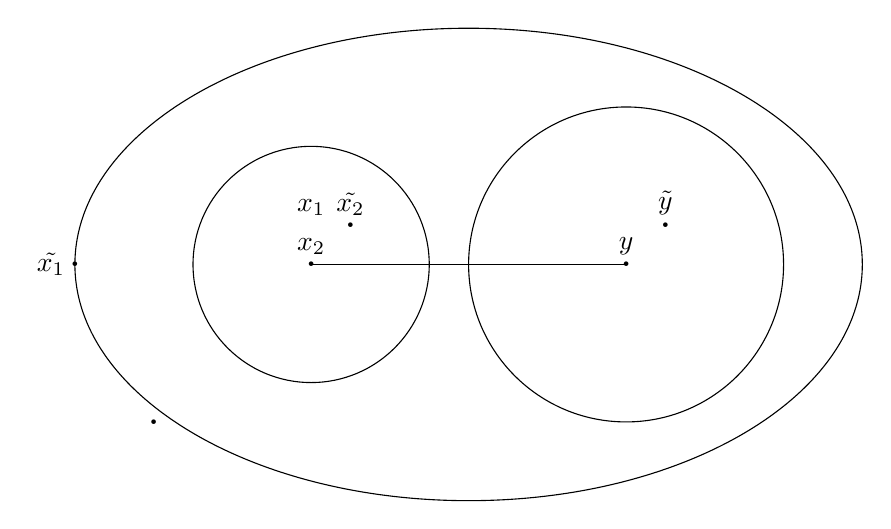
\begin{tikzpicture}
\draw (2,2) circle (1.5cm);
\draw (6,2) circle (2cm);
\draw (4,2) ellipse (5cm and 3 cm);
\draw (2,2) -- (4,2) -- (6,2);
\draw (6,2) node[point,above]{$y$};
\draw (6.5,2.5) node[point,above]{$\tilde{y}$};
\draw (2,2) node[point,above]{$x_2$};
\draw (2.5,2.5) node[point,above]{$\tilde{x_2}$};
\node[point,above] at (2,2.5) {$x_1$} ;
\draw (-1,2) node[point,left]{$\tilde{x_1}$};
\end{tikzpicture}
\end{figure}


A continuación, vamos a repasar un par de conceptos topológicos para demostrar:

\begin{corol}
Si $S\subset\mathbb{R}^n$ es convexo, entonces tanto $\mbox{int}(S)$ como $\bar{S}$ son conjuntos convexos.
\end{corol}
\begin{proof}
\textcolor{red}{Por hacer.}
\end{proof}
\begin{corol}
Si $S\subset\mathbb{R}^n$ es convexo, entonces $\mbox{int}(S)=\mbox{int}(\bar{S})$. 
Si además $\mbox{int}(S)\neq \emptyset$, entonces $\bar{S}=\overline{\mbox{int}(S)}$.
\end{corol}
\begin{proof}
\textcolor{red}{Por hacer.}
\end{proof}

\begin{corol}
Si $S\subset\mathbb{R}^n$ es convexo, entonces $\partial S=\partial \bar{S}$.
\end{corol}
\begin{proof}
\textcolor{red}{Por hacer.}
\end{proof}


\begin{theorem}[Teorema\IS de la proyección]
 Sea $S\subset\mathbb{R}^n$ un conjunto convexo, no vacío y cerrado. Sea $y\in \mathbb{R}^n$. Existe un \textbf{único} $\bar x\in S$ (la proyección de $y$ sobre $S$) tal que 
\[
\|y-\bar x\| \leq \|y - x\|, \ \ \mbox{para todo}\ x\in S.
\]
Además, $\bar x$ es la proyección de $y$ sobre $S$ si y solo si
\begin{equation}
\label{eq.proyeccion}
(y-\bar x)^\top (x - \bar{x}) \leq 0.
\end{equation}
\end{theorem}

\begin{proof}
$\gor{x} + λ(x-\gor{x})\in S$ por convexidad, $∀λ\in(0,1]$.

Además, tenemos que 

\[
||y-\vx||^2 \leq ||y-\vx - λ(x-\vx)||^2 = \norm{y-\vx}^2 + \norm{λ(x-\vx)}^2 + 2λ(x-\vx)^{t}(y-\vx)
\]

Reordenando y haciendo $λ\to 0$, entonces \[ (x-\vx)^{t}(y-\vx) \leq 0 \]

Hasta ahora, hemos encontrado que existe un punto y además, que cumple la condición. Ahora vamos a ver que es \textbf{único}. Es interesante que este truco, que se utilizará en algunos ejercicios.

Supongamos que existe $z\in S$ que cumple la condición, es decir: \[ (x-z)^{t}(y-z) \leq 0 \; ∀x\in S\]

El truco está en tomar $x = \gor x$, el punto que encontramos antes. Vamos a escribir las ecuaciones que tenemos.

\[ 
\begin{array}{c}
(y-\vx)^{t}(x-\vx) \leq 0 \\
(y-z)^{t}(x-z) \leq 0 \\
(z-y)^{t}(z-\gor{x}) \leq 0
\end{array}
\]


Ahora, si sumamos las 3, por alguna razón obtenemos: 

\[(z-\vx)^t(z-\vx) = \norm{z-\vx} \leq 0 \to z = \vx\]

\end{proof}

Vamos a profundizar un poco en el resultado de este teorema:
\textbf{¿Cómo queda la condición (\ref{eq.proyeccion}) cuando $S$ es un conjunto afín?}
La aplicación $P:\mathbb{R}^n\to S$, que a cada $y$ le hace corresponder su proyección $P(y)$ sobre $S$, es continua.

\subsection{Teoremas de separación}

\begin{theorem}[Teorema\IS del hiperplano separador]

Sea $S\subset\mathbb{R}^n$ un conjunto convexo, no vacío y cerrado. Sea $y\notin S$.
Entonces $\exists p\in\mathbb{R}^n$, $p\neq 0$, y $\exists\alpha\in\mathbb{R}$ tales que el punto está a un lado, y el conjunto al otro, es decir $p^\top x\leq \alpha$, para todo $x\in S$ y $p^\top y > \alpha$.

\end{theorem}


\begin{proof}
Sea $\gor{x}$ la proyección de $y$ sobre $S$ y definimos $p = y-\gor{x}$ y $\alpha = p^t\gor{x}$.

\[
p^tx = \underbrace{(y-\gx)^t(x-\gx)}_{\leq 0} + \underbrace{p^t\gx}_{0} \leq \alpha
\]

Por el otro lado,

\[
p^tx = \underbrace{(y-\gx)^t(y-\gx)}_{\norm{y-\gx}^2 > 0} + \underbrace{p^t\gx}_{\alpha} > \alpha
\]


Como vemos, esta demostración se basa en el teorema de la proyección.
\end{proof}


Sobre este teorema hay diversas versiones, dependiendo de las condiciones impuestas. Si en vez de considerarlo cerrrado lo consideráramos abierto, obtendríamos separación no estrcita. En este curso, utilizaremos únicamente esta versión del teorema.


\begin{theorem}[Teorema\IS hiperplano separador]
Sea $S\subset\mathbb{R}^n$ un conjunto convexo\footnote{En las diapositivas de la asignatura se incluye la condición de interior no vacío. Esta condición, en realidad no es necesaria porque cuando el interior es vacío, es un poco absurdo de aplicar, pero el teorema es cierto}. 
Sea $\bar{x}\in \partial S$, la frontera de $S$. 

Entonces existe $p\in\mathbb{R}^n$, $p\neq 0$, tal que $p^\top (x-\bar{x})\leq 0$, para todo $x\in S$.

\end{theorem}



\begin{proof}

Vamos a aplicar el teorema anterior. Como el punto $x$ está en la frontera, podemos acercarnos a él desde fuera. 
Si tenemos una sucesión de puntos $y_i$ que convergen a $x$, tenemos un hiperplano separador en cada $y_i$. Tomando límite, ese será el hiperplano soporte.

Sea $\gx \in \partial S = \partial\gor{S}$. Además, $\int{S} = \int{\gor{S}}$

\[∀k\in \nat \exists y_k \in B\left(\gx,\frac{1}{k}\right) \cap \gor{S}^C\]
Por el teorema del hiperplano separador (\ref) existe $p_k$ con $\norm{p_k}$ tal que $p^t y_k > p^t x$ por el teorema anterior, $∀x\in S$.

Como $\{ p : \norm{p}\}$ es un conjunto compacto, existe una subsucesión  de $p_k$  convergente a $p$.

Haciendo $k\to \infty$, perdemos la desigualdad estricta y obtenemos:

\[p^t\gx \geq p^tx \dimplies p^t(x-\gx) \leq 0\]

\end{proof}


\begin{theorem}[Teorema\IS de separación entre 2 convexos]

Sean $S_1,S_2\subset \real^n$ convexos no vacíos y tal que $S_1\cap S_2  =\emptyset$.

\textbf{Entonces} existe $p\in\real^n$, con $p≠0$ tal que:

\[
\inf{p^tx: x\in S_1} \geq \sup\{p^tx : x\in S_2\}
\]

\end{theorem}

\begin{proof}
La demostración es un ejercicio de la hoja.

Tomando $S = \{x\in\real^n: x = x_1 - x_2, x_i \in S_i\}$.

$S$ es convexo y $0 \not\in S$.

Si $0\in\gor{S}$, aplicamos el primer teorema. Si $0\in\partial{S}$, aplicamos el segundo teorema
\end{proof}


\obs Aunque $S_1$ y $S_2$ sean cerrados, la desigualdad no tiene porqué ser estricta.




\subsection{Teoremas de la alternativa}

Ahora que ya hemos visto muchos conceptos generales, vamos a volver a los problemas de optimización.
Una buena herramienta son estos teoremas, que nos ayudan a saber si un sistema tiene solución o no.

\begin{lemma}[Lema\IS de Gordan]
Sea $A$ una matriz $m\times n$. Entonces, uno y \textbf{sólamente uno} de los siguientes sistemas tiene solución.

\begin{equation}
Ax < 0\;,\; x\in\real^n
\label{eq:Gordan_1}
\end{equation}

\begin{equation}
A^tp = 0\;,\; p > 0
\label{eq:Gordan_2}
\end{equation}
\end{lemma}


Vamos a razonar geométricamente, qué tiene que ocurrir para que los 2 sistemas tuvieran solución. Sea $A = (a_1^t,a_2^t)^t$.

\begin{figure}[h]
\centering
\begin{tikzpicture}
\draw (-2,0) -- (2,0);
\draw (0,-2) -- (0,2);
\draw[->] (0,0) -- (1,0) node[above] { $a_1$ }; 
\draw[->] (0,0) -- (-1,0) node[above] { $a_2$ }; 
\end{tikzpicture}
\end{figure}

En este caso, tenemos \[Ax < 0 \dimplies \left.\begin{array}{c}a_1^tx < 0\\a_2^tx<0\end{array}\right\} \to a_1 = -\alpha a_2\]


Por alguna razón que no se muy bien, vemos que $A^tp$ no tiene solución.


Antes de meternos con la demostración del teorema, vamos a ver qué relación tiene este resultado con los problemas de optimización que se supone que queremos aprender a resolver en esta asignatura.
Pensemos en el problema:
\begin{ioprob}
\goal{$\min f(x)$}
\restrictions{$g(x) \leq 0$}{}{}{}{}{}
\end{ioprob}

$\gor{x}$ es el mínimo local del problema $\dimplies$
\[\left.\begin{array}{c}\not\exists d \tq \grad f(\gx)^td < 0 \\ \grad g(\gx)^td < 0\end{array}\right\} \to \exists p = \begin{pmatrix}p_1\\p_2\end{pmatrix} \tq p_1\grad f(\gx) + p_2 \grad g(\gx) = 0, p_i \geq 0\]

\begin{proof}
La parte fácil es la demostración de: \ref{eq:Gordan_1} tiene solución, entonces \ref{eq:Gordan_2} no tiene solución.

Sea $\gx$ la solución de \ref{eq:Gordan_1} y supongamos que $\gor{p}$ es la solución de \ref{eq:Gordan_2}.

Consideremos:
\[\gor{p}^t A \gx = \underbrace{\gor{p}^t(A\gor{x})}_{<0} = \underbrace{(A^t\gor{p})^t\gor{x}}_{=0}\]

No puede ser igual y menor que 0 al mismo tiempo.


Vamos a ver que si \ref{eq:Gordan_1} no tiene solución, entonces \ref{eq:Gordan_2} sí la tiene. Aquí es donde entran los teoremas de separación.

Sean \[S_1 = \{z\in\real^m: z=Ax, x\in\real^n\}\subset\real^m\]
 \[S_2 = \{z\in\real^m: z<0\}\subset\real^m\]

Estos 2 conjuntos son convexos\footnote{¿Por qué?} y por otro lado, $S_1 \cap S_2 = \emptyset$, ya que \ref{eq:Gordan_1} no tiene solución.

Vemos que $\exists p ≠ 0$ tal que $p^tAx \geq p^tz, \forall x\in\real^n,z<0,z\in\real^m$


$p$ resuelve \ref{eq:Gordan_2}. Supongamos que $p\not\geq0$ (por ejemplo $p_j < 0$).

Consideramos: $z = -\lambda (0,\cdots,0,1,0,\cdots,0)$, con $\lambda > 0$.

Entonces, $p^tAx \geq -\lambda p_j \convs[λ\to\infty]\infty$ y esto se da $\forall x\in\real^n$

$x = -A^tp \to p^tAx = -\norm{A^tp}^2 \leq 0$

Pero haciendo $z\to 0$, resulta que $p^tAx \geq 0 \forall x \implies -\norm{A^tp}\geq 0$.

Como $\norm{A^tp} \geq 0$ y $\norm{A^tp} \leq 0$, deducimos que $\norm{A^tp} = 0$, con lo que \ref{eq:Gordan_2} tiene solución.
\end{proof}


























\chapter{Condiciones KKT y dualidad}
% -*- root: ../InvestigacionOperativa.tex -*-

\section{Introducción}

En esta sección, vamos a repasar conceptos y algunas aplicaciones porque de aquí en adelante trabajaremos con estos conceptos.


\begin{itemize}
	\item Gradiente.
	\item Matriz Hessiana.
	\item Desarrollo de Taylor en varias variables:
		\[
			f(\vx) = f(\gor{\vx}) + \grad f(\gor{\vx})^\top (\vx-\gor{\vx}) + (\vx-\gor{\vx})\Hf{\gor{\vx}}(\vx-\gor{\vx}) + \norm{\vx-\gor{\vx}}R(\gor{\vx},\vx-\gor{\vx})
		\]
		con $\displaystyle \lim R(\vx,\gor{\vx}) = 0$ ($R$ es el resto).
\end{itemize}

\subsection{Condiciones para óptimos locales}

\paragraph{Condición necesaria de primer orden}
Si $\vx$ es un máximo o mínimo local, entonces $\grad f(\vx) = 0$.

Para ver que la condición es necesaria pero no suficiente, podemos pensar en $f(x_1,x_2) = x_1^2 - x_2^2$, cuyo gradiente se anula en $(0,0)$, pero no es un mínimo ni un máximo. Estamos ante un punto de silla (punto de inflexión).


\paragraph{Condiciones necesarias de segundo orden} Sea $f$ 2 veces diferenciable en $\gor{\vx}$. Si $\gor{\vx}$ es un mínimo local de $f$, encones:
\begin{itemize}
	\item $\grad f(\gor{\vx}) = 0$
	\item $\Hf{\gor{\vx}}$ semidefinida positiva.
\end{itemize}

Con el mismo ejemplo anterior podemos ver que es condición necesaria.

\paragraph{Condiciones suficientes} Sea $f$ 2 veces diferenciable en $\gor{\vx}$. Si $\gor{\vx}$ es un mínimo local de $f$, encones:
\begin{itemize}
	\item $\grad f(\gor{\vx}) = 0$
	\item $\Hf{\gor{\vx}}$ definida positiva.
\end{itemize}
\begin{proof}
	Si $\vx$ no es un mínimo local estrico, entonces existe una sucesión $\vx_k \to \gor{\vx}$ con $\gor{\vx_k} ≠ \vx$ tal que $f(\vx_k) ≤ f(\gor{\vx})$.

	Sea \[d_k = \frac{\vx_k - \gor{\vx}}{\norm{\vx_k - \gor{\vx}}}\]

	Las normas están acotadas, y estamos en $\real^n$ y algún argumento de compacidad, podemos tomar una subsucesión convergente de $d_k\to d$, que vamos a llamar $d_k$

	Tomamos el desarrollo de Taylor de $f(\vx_k)$:

	\[
		f(\vx_k) = f(\gor{\vx}) = f(\gor{\vx}) + \frac{1}{2}\Hf{f(\gor{\vx})}(\vx_k - \gor{\vx}) + \norm{\vx_k - \gvx}^2R(\gx,\gx_k)
	\]

	\[
		0≥\frac{f(\vx_k - f(\gx)}{\norm{\vx_k - \gvx}^2} = \frac{1}{2}d_k^t\Hf{f(\gvx)}d_k + R(\gvx,\vx_k)
	\]
	Hemos llegado a que $\Hf{f(\gvx)}$ tiene que ser semidefinida negativa.
\end{proof}

Estas condiciones están bien, pero no son del todo interesantes para este curso, ya que estamos buscando soluciones globales a problemas y todas estas condiciones son locales.
Vamos a necesitar alguna restricción más sobre $f$ para poder buscar soluciones globales.

\subsection{Funciones convexas}

\begin{defn}[Función\IS convexa]
Una función $\appl{f}{D}{ℝ}$ es convexa si su dominio $D\subset\real ℝ^n$ es covexa y  $∀\vx,\vy\in D$, $∀λ∈[0,1]$ se verifica:

\[
	f(λ\vx + (1-λ)\vy ≤ λf(\vx) + (1-λ)f(\vy)
\]
\end{defn}

\obs
\begin{itemize}
	\item \concept{Convexidad\IS estricta} requiere $<$ en lugar de $≤$.
	\item Una función es (estrictamente) cóncava si $-f$ es (estrictamente) convexa.
	\item $f$ es convexa $\dimplies ∀x,\vec{u}, g(t) = f(x+tu)$ es convexa (en su dominio, es decir $\{t : x+tu\in D\}$)
	\begin{proof}
		\[g(λt_1+(1-λ)t_2) = f(x+(λt_1+(1-λt_2)\vu) = ...
		\]
	\end{proof}
\end{itemize}

\begin{example}
\begin{itemize}
	\item $f(x) = x^2$ es convexa.

	Como todavía no hemos visto la definición de convexidad en términos de la segunda derivada, vamos a recurrir a la definición.
	\begin{proof}
		\[
			\left(λx_1 + (1-λ)x_2\right)^2 ≤ λx_1^2 +(1-λ)x_2^2)
		\]
	\end{proof}
	\item $f(\vx) = \max\{x_1,...,x_n\}$ es convexa.
	\begin{proof}
		\[f(λ\vx + (1-λ) \vy) = \max\set{λx_1 + (1-λ)y_1,...,λx_n + (1-λ)y_n} ≤ λ\max\{x_k\} + (1-λ)\max\{y_k\} = λf(\vx) + (1-λ)f(\vy)\]
	\end{proof}
	\item Las funciones afines $f(x) = A\vx + b$ son cóncavas y convexas.
	\item Cualquier norma $f(\vx) = \norm{\vx}$ es una función convexa.
	\item Si $S$ es convexo, la distancia a $S$:
	\[
		f(x) = d(x,S) = \inf_{s\in S}\norm{\vx-s}
	\]
	es una función convexa.

\end{itemize}

\begin{theorem}[Desigualdad\IS de Jensen]
Si $\appl{f}{D}{ℝ}$ es convexa, entonces $∀x_1,...,x_n\in D$ y $,λ_1,...,λ_n ≥0$ con $\sum^n λ_i = 1$ se cumple:

\[f\left(\sum^k x_iλ_iy\right) ≤ \sum^k λ_if(x_i)\]

\end{theorem}
\begin{proof}
Por inducción sobre $k$.
\end{proof}

\obs Podríamos interpretar $λ_i$ como probabilidades y tendríamos:

Si $X$ es una variable aleatoriao que toma los valores $x_i$ con probabilidad $λ_i$, entonces $f(\esp{X})≤\esp{f(X)}$

\end{example}

Vamos a ver más condiciones de convexidad de funciones, para no tener que recurrir a la definición.

\paragraph{Completar la teoría}


\paragraph{Ejemplos}
\begin{itemize}
	\item $f(x) = -\log(x)$ podemos derivar 2 veces y como es positiva, convexa.
	\item $f(x) = e^{ax}$ es convexa.
	\item $f(x) = x^a$
	\subitem $a≤0, a≥1 \to$ convexa.
	\subitem $0<a<1 \to $ cóncava.
	\item $f(x) = x^\top Ax + a^\top x+ c$ donde $A$ es simétrica. Queremos ver que $f$ convexa $\dimplies$ $A$ definida positiva.
	\item La más relevante: $X$ una matrix $n\times p$ y sean $β\in\real^p$ e $y\in\real^n$, entonces:
	$f(β) = \norm{y-Xβ}$ es convexa, siendo $\norm{·}$ cualquier norma.

	Esta función es convexa porque es la composición de 2 funciones. $Xβ$ es una función afín y la norma es convexa para cualquier norma. Entonces, como $f(β)$ es una combinación de funciones convexas, es convexa.
\end{itemize}



\section{Cuasiconvexidad}


Aquí faltan bastantes cosas.


\subsection{Utilidad}

La cuasiconvexidad es una propiedad más relajada que al convexidad pero que es condición suficiente para algunos resultados interesantes. Por ejemplo:

\begin{prop}
Mínimo local en función cuasiconvexa es un mínimo global.
\end{prop}

\begin{proof}
Se deja como ejercicio
\end{proof}




\section{Tras la reparación}

\subsection{Resumen}

\begin{table}[hbtp]
\centering
\begin{tabular}{c|c|c}
Primal $\equiv$ (P) & $\begin{array}{c} \min c'x\\Ax = b\\x≥ 0\end{array}$ & $\begin{array}{c} \max c'x\\Ax ≤ b\\x≥ 0\end{array}$\\
\hline
Dual $\equiv$ (D) & $\begin{array}{c} \max b'u\\A'u ≥ c\end{array}$ & $\begin{array}{c} \max b'u\\A^\top u ≤ c\\u≥ 0\end{array}$\\
\end{tabular}
\caption{Resumen de pasar del problema primal al dual.}
\end{table}


\subsection{Interpretación económica del problema dual}

La solución del problema dual del pastelero es $u = \left(\rfrac{1}{3},0,10\right)$, que son los valores que aparecían en el problema \ref{ejer:pastelero}. Además, vemos también que $\bar{p} = \bar{d} = 775$. Es decir, la dualidad es fuerte. 

Vamos a demostrarlo teóricamente.


\begin{defn}[Dualidad\IS fuerte]
$\bar{p} = \bar{d}$
\end{defn}


\begin{example} Escribe el dual de:

...

\begin{ioprob}
\goal{$\min -u_1 - u_2$}
\restrictions{$-u_2≥1$}{$u_2 ≤ 1-$}{$u_1-u_2≥-1$}{$u_1 ≥$}{$u_2≥0$}{}
\end{ioprob}

Aquí no tienen solución ni el factible ni el primal.
\end{example}

\begin{theorem}[Dualidad fuerte para problemas lineales]

Consideremos un problema lineal en forma estándar $(P)$ y el correspondiente problema dual $(D)$. 

Si $(P)$ tiene solución factible óptima finita, también la tiene $(D)$ y los correspondientes valores óptimos son iguales.
\end{theorem}

\begin{proof}
\[u' \equiv c_B'B^{-1}\]

\[
\begin{array}{c}
u'b = c'_BB^{-1}b
c'x = c'_BB^{-1}n]c_N'0
\end{array}
\]


$u$ es factible para $(D)$ $\dimplies$ 

\[u'A ≤ c' = c'_BB^{-1}\left(B | N \right) ≤ (c'_B,c'_N)\dimplies \underbrace{c_B'B^{-1}N}_{z_j} ≤ c'_N\]

Demostrar que $u$ es factible es lo mismo que demostrar que $z_j ≤ c_j$ en la tabla del simplex. Como $\bar{x}$ es el óptimo, en la última fila de simplex tenemos todos $≤0$, con lo que $z_j ≤ c_j$

\paragraph{Conclusión: } Encontrar un óptimo para el primal es encontrar un factible para el dual.

\end{proof}



\[
\dpa{\bar{z}}{b_i} = u_i
\]
Esto demuestra la observación de que la solución del dual del pastelero corresponde al beneficio marginal que gana de más al aumentar en 1 su cantidad de azúcar/mantequilla/harina. Esto es general para cualquier problema lineal.





\subsection{Algortimo simple-dual}

Tenemos un problema de programación lineal que resolvemos con simplex normal. Llegamos a una solución óptima que es factible del dual. Ahora, imaginemos que cambiamos $b$, con lo que las restricciones dejan de cumplirse. El estado de la tabla del simplex se mantiene, salvo la columna de la izquierda. 
Este es un punto de partida para este algoritmo. Otro caso ventajoso de este algoritmo se da al tener ¿coeficientes negativos?


\paragraph{Completar de las traspas}


\begin{example} Resolver el problema:

...

Lo primero es pasarlo a forma estándar:


\begin{ioprob}
\goal{$\min{3x_1 + 2x_2}$}
\restrictions{$3x_1-x_2+x_3 = -3$}{...}{...}{...}{...}{...}
\end{ioprob}


En este caso, no podemos empezar con el algoritmo del simplex, porque hay $b_i< 0$. Pero tendríamos una solución óptima si fuera factible. Al ser óptima en el primal, es factible en el dual y podemos aplicar el algoritmo del simplex-dual.
Vamos a ver la evolución de las tablas.


\paragraph{Vamos a verlo gráficamente paso a paso}

\begin{figure}[hbtp]
\centering
\begin{tikzpicture}[scale=1.5]
\draw[thick,->] (0,0) -- (3.5,0);
\draw[thick,->] (0,0) -- (0,3.5);
\draw[thick,-] (3,0) -- (0,3);
\draw[thick,-] (1,0) -- (0,3);
\draw[thick,-] (1.5,0) -- (0,2);
\filldraw[fill=blue, opacity = 0.4] (3/5,6/5) -- (1.5,0) -- (3,0) -- (0,3) -- cycle;
\node [label={below:$(1)$},nodepoint, inner sep=2pt,color=red] at (0,0) {};
\node [label={left:$(2)$},nodepoint, inner sep=2pt,color=blue] at (0,2) {};
\node [label={below left:$(3)$},nodepoint, inner sep=2pt,color=green] at (3/5,6/5) {};
\end{tikzpicture}
\caption{Evolución del algoritmo del simplex-dual.}
\end{figure}


\end{example}

\chapter{Aplicaciones}
\section{Máquinas de vectores soporte}

\paragraph{Introducción}

Para más información sobre la clasificación, consultar el último capítulo de \citep{ApuntesEstII}.
%

Disponemos de una muestra de datos bien clasificados (\textit{training data}):

\[
(x_1,y_1),\ldots, (x_n,y_n)
\]
donde $x_i\in \mathbb{R}^d$ son las variables observadas e $y_i\in\{-1,1\}$ es la etiqueta que representa la clase a la que pertenecen las observaciones.

\

Se observa ahora un nuevo vector $x$ independiente de los anteriores.

El objetivo es determinar a qué clase pertenece la observación $x$.

\

La regla óptima (regla Bayes) consiste en asignar a $x$ el valor $y=1$ si y solo si
\[
\mathbb{P}(y=1| x) > \mathbb{P}(y=-1|x)
\]
No es aplicable en la práctica, con lo que necesitamos buscar otros sistemas. 
%
A lo largo de este tema vamos a estudiar una regla de clasificación basada en contenidos anteriores del curso.

\paragraph{SVM para datos separables}

Suponemos que las muestras de ambos grupos son separables mediante un hiperplano:

\begin{figure}[hbtp]
\centering
\includegraphics[scale=0.7]{img/margen}
\caption{Datos separables}
\end{figure}

El \concept{margen} de un hiperplano separador viene dado por la menor distancia de los puntos al hiperplano. 

El \concept{hiperplano óptimo} es aquel que maximiza el margen.


Dada una muestra de datos $(x_i,y_i)$, para poder clasificarla necesitamos encontrar ese hiperplano separador.
%
Definimos las clases $y_i\in\{-1,1\}$. Entonces, un hiperplano separador verifica $y_i(ω'x_i+ω_0)>0$.
%
Si es de clase $y_i=-1$, entonces $(ω'x_i + ω_0) < 0$ y viceversa.

Pdemos definir $ω$ y $ω_0$ de manera que  $\min_i \{y_i(w' x_i + w_0)\}=1$
con lo que el margen es: $\mbox{Margen} = \min_i  \frac{y_i(w' x + w_0)}{\|w\|} = \frac{1}{\|w\|}$.


\paragraph{Cálculo de hiperplano óptimo}


Para buscar el hiperplano óptimo, que es aquel que maximiza el márgen. Entonces, el problema de optimización asociado es:

\begin{ioprob}
\goal{$\min \frac{\norm{ω}^2}{2}$}
\restrictions{$y_i(ω'x_i + ω_0) ≥ 1$}{}{}{}{}{}
\end{ioprob}


Al resolver este problema, por la holgura complementaria, llegamos  a que el óptimo sólo depende de los puntos en los que $u_i≠0 \to y_i(ω'x_i + ω_0) = 1$, es decir, en la frontera.

\subparagraph{Cálculo del dual}
Vamos a estudiar el problema dual del planteado aquí.

\[
	g(u) = \frac{1}{2} \underbrace{\left(\sum_i y_iu_ix_i\right)^\top}_{ω} \underbrace{\sum_jy_ju_jx_j}_{ω} - \sum u_jy_jx_j\right)^\top x_i - \left(\sum y_ju_j\right)ω_0 + \sum u_i = \sum_{i=1}^n u_i - \frac{1}{2} \sum_{i=1}^n \sum_{j=1}^n  u_i u_j y_i y_j x'_i x_j 
\]

Con lo que:

\[
	g(u) =\begin{array}{ccc} -∞ & si &\sum y_iu_i ≠ 0\\ \sum u_i - \frac{1}{?}\sum_i\sum_j u_i u_j y_i y_j x'_i x_j  & si & \sum y_iu_i = 0
	\end{array}
\]

Vamos a expresar el problema dual.
%
Tomando $\vec{1} = (1,...,1)$, y $H = (h_{ij}) = (y_iy_jx'_ix_j)$

\begin{ioprob}
\goal{$\max \vec{1}^\top u - \frac{1}{2}\vec{u}^\top H\vu$}
\restrictions{$\vy^\top \vu = 0$}{$u≥0$}{}{}{}{}
\end{ioprob}

¿Es este problema convexo? Para poder contestar necesitaríamos que $H$ sea semidefinida positiva. 
%
Esto es cierto porque:

\[
	\vu'H\vu = \norm{\sum ...}^2 ≥ 0
\]


Como $H$ es semidefinida positiva, tenemos un problema convexo. \todo{¿Porqué?}

Además, \textbf{la solución depende} de $x_1,\ldots,x_n$ \textbf{únicamente a través de los productos escalares} $x'_ix_j$.


\subparagraph{Holgura complementaria}

A partir de la solución del dual, $\hat u$, aplicamos $\hat w = \sum_{i=1}^n \hat u_i y_i x_i$ para obtener $\hat w$.

 Sean $S=\{i:\, \hat u_i>0\}$ los índices de los vectores soporte.
Por las condiciones de holgura complementaria,  para cada $i\in S$,
\[
\hat w_0 = \frac{1-y_i\hat w'x_i}{y_i} = y_i-\hat w'x_i.
\] 


En la práctica, es numéricamente más estable usar el promedio de estos valores. Si $\# S=n_s$.
\[
\hat w_0 = \frac{1}{n_s} \sum_{i\in S} (y_i-\hat w'x_i).
\]

\subsubsection{Regla de clasificación}

Resulta una regla de clasificación lineal: asignamos a $x$ el valor $y=1$ si y solo si $\hat{w}'x+\hat w_0>0$.

\

\[
\hat w_0 + \hat{w}'x>0 \Leftrightarrow \hat w_0 + \left[\sum_{i\in S} y_i \hat u_i x_i\right]' x > 0 
\]

\

Si $\alpha_i=y_i\hat u_i$, también podemos escribir la regla de clasificación como:
\[
y = 1 \Leftrightarrow  \hat w_0 + \sum_{i\in S} \alpha_i (x'_ix)>0
\]

¿Cómo afecta a la clasificación una rotación de los datos?

Tomamos $\tilde{u}_i = Cu_i$, siendo $C$ ortonormal. 
%
Repasando los cálculos anteriores con $\tilde{u}_i$ obtenemos que $\tilde{ω} = Cω$, es decir, el hiperplano óptimo de los datos rotados es la rotación del hiperplano óptimo.

\paragraph{SVM datos no separables}

En la realidad, los datos separables no son habituales. 
%
El truco es añadir una penalización a los puntos que están mal clasificados (o demasiado cerca del hiperplano). Es decir:

\[
	y_i(ω'x_i + ω_0) ≥ 1-\xi_i
\]

¿Cuánto penalizamos la distancia? Eso se refleja con una constante $C$, de la siguiente manera:

\begin{ioprob}
\goal{$\|w\|^2 / 2 + C\sum_{i=1}^n \xi_i$}
\restrictions{$y_i(w' x_i + w_0) + \xi_i\geq 1\;\; i=1,\ldots,n$}{$\xi_i\geq 0\;\;i=1,\ldots,n$}{}{}{}{}
\end{ioprob}

Y ahora, para construir la regla de clasificación damos los mismos pasos que en el caso de datos separables linealmente. 
%
Estos son: $KKT$, problema dual, holgura complementaria.

\todoby{dejuan}

Llegamos al problema dual:


\begin{ioprob}
\goal{$\max g(u) = \vec{1}'\vu - \rfrac{1}{2}\vec{u}'H\vu$}
\restrictions{$\vu'y = 0$}{$C≥u≥0$}{}{}{}{}
\end{ioprob}

La única diferencia que aparece es $C≥u$, es decir, los pesos están acotados superiormente.


%% Apéndices (ejercicios, exámenes)
\appendix

\chapter{---}
 %-*- root: ../InvestigacionOperativa.tex -*-

\section{Hoja 1}

\begin{problem}[1]

Una empresa de reciclaje usa papel y tela desechados para fabricar dos tipos distintos de papel reciclado.
Cada tanda de papel reciclado de clase A requiere 20 kg de tela y 180 kg de papel y produce un beneficio de 500 euros, mientras que cada tanda de papel reciclado de clase B requiere 10 kg de tela y 150 kg de papel y produce un beneficio de 250 euros. 
La compañía dispone de 100 kg de tela y 660 kg de papel. ¿Cuántas tandas debe fabricar de cada tipo?

\solution

\begin{center}
\begin{tabular}{c|ccc}
& A & B & Disp. \\\hline
Tela & 20 & 10 & 100\\
Papel & 180 & 150 & 660\\
Beneficio & 500 & 250 & 
\end{tabular}
\end{center}

Variables $x = $ calidad de A e $y = $ calidad de B.

\begin{ioprob}
\goal{$\max 500x_1 + 250 x_2$}
\restrictions{$20x_1 + 10x_2 \leq 100$}{$180x_1 + 160x_2 \leq 660$}{$x_i \geq 0$}{}{}{}
\end{ioprob}

Vamos a resolverlo gráficamente en la figura \ref{ej:1.1.a}. Vamos a reprensentar el conjunto del plano que cumple las 3 restricciones.


\begin{figure}[hbtp]
\centering
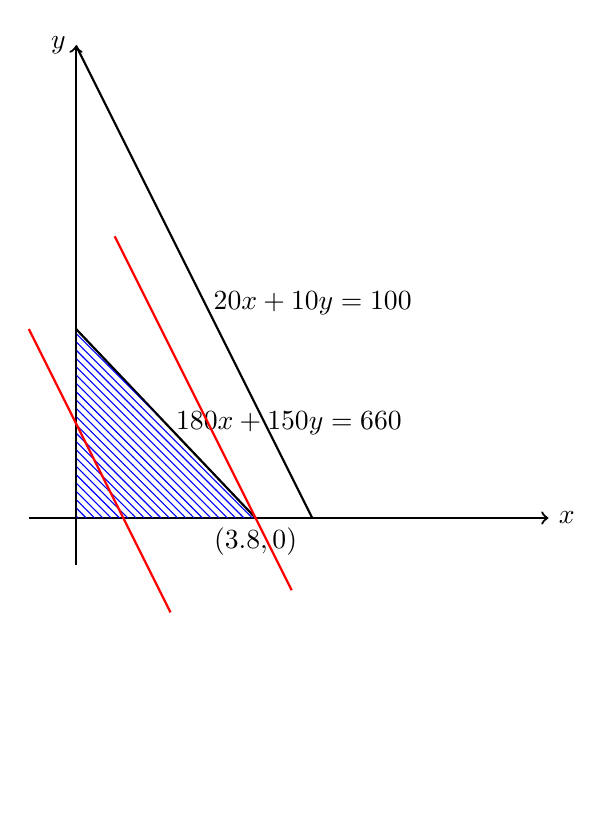
\begin{tikzpicture}[scale=0.6]
\draw[thick,->] (-1,0) -- (10,0) node[anchor=west] {$x$};
\draw[thick,->] (0,-1) -- (0,10) node[anchor=east] {$y$};
\draw[thick,-] (5,0) -- node[anchor=north west] {\text{ }$20x + 10 y = 100$} (0,10);
\draw[thick,-] (3.8,0) -- node[anchor=west] {$180x + 150y = 660$} (0,4);
\filldraw[fill=blue!40!white, pattern=north west lines, pattern color=blue] (0,0) -- (0,4) -- (3.8,0);
\draw[thick,-,color=red] (2,-2) -- (-1,4);
\draw (3.8,0) node[anchor=north]  {$(3.8,0)$};
\draw [shorten >= 3cm, shorten <= -4cm,color=red,thick] (3.8,0) -- +($(2,-2)-(-1,4)$);
\end{tikzpicture}
\label{ej:1.1.a}
\caption{Representamos las 2 rectas fronteras y el vector gradiente de la función objetivo.}
\end{figure}


La idea es mover la recta roja en su dirección perpendicular todo lo que podamos. En este caso, no podremos alejarnos más que el punto que del punto $(3.8,0)$, con lo que será el óptimo.

\end{problem}


\begin{problem}[2]

La empresa Animales Salvajes S.A. cría faisanes y perdices para repoblar el bosque y dispone de sitio para criar 100 pájaros durante la temporada.
Criar un faisán cuesta 20 euros y criar una perdiz cuesta 30 euros. 
La fundación Vida Animal paga a Animales Salvajes S.A. por los pájaros de forma que se obtiene un beneficio de 14 euros por cada faisán y 16 euros por cada perdiz. 
La empresa dispone de 2400 euros para cubrir costes. ¿Cuántas perdices y cuántos faisanes debe criar?


\solution 


\begin{center}
\begin{tabular}{c|cccc}
&Faisán & Perdiz & Disp. & \# pájaros \\\hline
Coste&20&30&2400&100\\
Beneficio&14&16&
\end{tabular}
\end{center}

Las variables utilizadas son $x$ para Faisán e $y$ para Perdiz.

El problema a resolver sería:

\begin{ioprob}
\goal{$\max 14x + 16y$}
\restrictions{$x+y\leq 100$}{$20x + 30y \leq 2400$}{$x,y > 0$}{}{}{}
\end{ioprob}

En la figura \ref{ej:1.2.a} encontramos la solución gráfica del problema. Vemos que la solución es la intersección de las rectas, así que calculamos la intersección: 
\[
\left.
	\begin{array}{cc}
		x+y = 100 \\ 
		20x+30y = 2400
	\end{array}
\right\} 
\to (x,y) = (40,60)
\]

\begin{figure}[h]
\centering
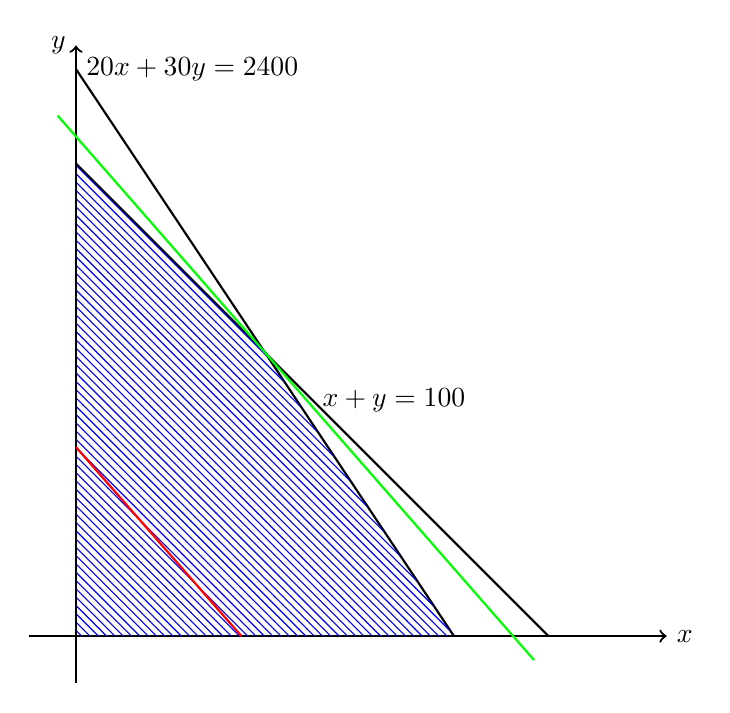
\begin{tikzpicture}[scale=0.6]
\draw[thick,->] (-1,0) -- (12.5,0) node[anchor=west] {$x$};
\draw[thick,->] (0,-1) -- (0,12.5) node[anchor=east] {$y$};
\draw[thick,-] (10,0) --  node[anchor=west] {$x+y=100$} (0,10);
\draw[thick,-] (8,0) -- (0,12) node[anchor=west] {$20x + 30y = 2400$};
\filldraw[fill=blue!40!white, pattern=north west lines, pattern color=blue] (0,0) -- (0,10) -- (4,6) -- (8,0);
\draw[thick,-,color=red] (3.5,0) -- (0,4);
%\draw[thick,-,color=green] (9,0) -- (0,11);
\draw [shorten <= -4cm,shorten >= -2cm, ,color=green,thick] (4,6) -- +($(3.5,0)-(0,4)$);
\end{tikzpicture}
\label{ej:1.2.a}
\caption{Representamos las 2 rectas fronteras y el vector gradiente de la función objetivo. En rojo la dirección del gradiente y en verde la solución óptima.}
\end{figure}





\end{problem}


\begin{problem}[3]

La siguiente tabla da el porcentaje de proteínas, grasas y carbohidratos, para cinco alimentos
básicos, A, B, C, D y E :


Los precios por 100 g de estos alimentos (dados en el mismo orden de la tabla) son 5, 17, 37, 10,
15. Si una persona necesita consumir como mínimo 75 gramos de proteínas, 90 de grasas y 300 de
hidratos de carbono, plantea el problema de minimización para calcular la dieta alimenticia de mínimo coste.
\solution


\end{problem}


\begin{problem}[9]

Una propiedad conocida de la mediana de un conjunto de datos $y_i$ es que minimiza en $\theta$ el valor de $\sum y_i-\theta$. Plantea el problema de optimización como un problema lineal en forma estándar.
\solution

Queremos minimizar 
\[\sum_{i=1}^n |y_i - \theta|\]

El procedimiento habitual podría ser derivar e igualar a 0, pero en este caso no podemos ir por ese camino, ya que no es derivable.
Vamos a ver que la solución es la mediana y vamos a demostrarlo de 2 maneras distintas. 
Primero, formalmente y después, planteándolo como un problema de optimización lineal.

\begin{proof}

Tomando una muestra de tamaño 2 y un punto interior de $\theta$ el objetivo a minimizar es:
\[\sum |y_i - \theta| = \theta - y_{(1)} + y_{(2)}-\theta = y_{(2)} - y_{(1)}\]
es decir, la longitud del intervalo.

Vamos a tomar una muestra de tamaño $n$. 
En esa muestra,tTomamos una serie de intervalos contenidos de la siguiente manera:

\[ [y_{(1)},y_{(n)}] \supset  [y_{(2)},y_{(n-1)}] \supset [y_{(3)},y_{(n-2)}] \supset ... \supset [y_{(m)},y_{(n-m+1)}]\]

Donde \[m=\left\{ \begin{array}{cc} \frac{n}{2} & n\text{ par}\\ ?? & n\text{ impar} \end{array}\right.\]
Este es un razonamiento casi geométrico de porque la mediana minimiza.
\end{proof}


Ahora, vamos a contestar al enunciado, planteándolo como un problema de regresión.

Definimos $x_i \equiv y_i - \theta = x_i^+ - x_i^-$ donde $x_i^+ = \max\{x_i,0\}$ y $x_i^- = \max\{-x_i,0\}$

De esta manera, $\abs{x_i} = x_i^+ + x_i^-$. Con este truco, hemos conseguido modificar la función objetivo, que de esta manera es una función lineal.

Nuestra función objetivo es:

\[\min \sum_{i=1}^n x_1^+ + x_i^-\]

Y el precio a pagar, es que necesitamos incluir una restricciones, con lo que:


\begin{ioprob}
\goal{\[\min \sum_{i=1}^n x_1^+ + x_i^-\]}
\restrictions{$y_i = x_i^+ - x_i^- + \theta^+ + \theta^-$, $i=1,...,n$}{$x_i^+ \geq 0$}{$x_i^- \geq 0$}{$\theta_i^+ \geq 0$}{$\theta_i^+ \geq 0$}{}
\end{ioprob}


Vamos a escribirlo matricialmente.
Las \textbf{variables de decisión} son $(x_1^+,...,x_n^+,x_1^-,...,x_n^-,\theta^+,\theta^-$. 

\[c = (\underbrace{1,...,1}_{n},\underbrace{1,...,1}_{n},0,0)\]
\[b = (y_1,...,y_n) \]
\[A = \left( I | -I | 1_n | -1_n\right)\to \begin{array}{c}1_n = \begin{pmatrix}1\\1\\\vdots\\1\end{pmatrix}\\ I = \text{ identidad} \end{array}\]




\obs{}
¿Qué utilidad puede tener esto?
Al tomar un modelo de regresión (una recta que pase por una nube de puntos) se suele tomar el criterio de "mínimos cuadrados", que es minimizar $\sum y_i-(β_0+β_1x_i)$ (siendo $β_0+β_1x$ el modelo de regresión). 
Podríamos plantear un modelo de regresión con otro criterio, por ejemplo, el de minimizar el valor absoluto.




\end{problem}



\section{Hoja 3}
\begin{problem}[1]
Sea $S\subset \real^n$. Dado $ε\geq 0$, la dilatacińo de $S$ se define como \[S_ε = \{x:d(x,S)\leq ε\}\] donde \[d(x,S) = \inf_{y\in S}{\norm{x-y}}\]

La erosión de $S$ se define como 
\[S_{-ε} = \{x:B(x,ε) \subset S \} \]

Demuestra que si $S$ es convexo, entonces tanto $S_{ε}$ como $S_{-ε}$ son conjuntos convexos

\solution
\doneby{Uceda}

\end{problem}


\begin{problem}[2]
Sean $x_0,...,x_k \in \real^n$. Considera los puntos que están más cerca de $x_0$ que de otro de los puntos $x_i$, es decir,

\[V = \{x\in\real^n : \norm{x-x_0}\leq \norm{x-x_i}\;,i=1,...,k\}\]

El conjunto $V$ se llama \textbf{región de Voronoi} de $x_0$ respecto de $x_1,...,x_k$

\ppart Demuestra que $V$ es un poliedro. Determina la matriz $A$ y un vector $b$ tales que $V = \{x\in\real^n Ax\leq b\}$

\ppart Recíprocamente, dado un poliedro $P$ con interior no vacío, determina $x_0,...,x_k$ de manera que $P$ sea la región de Voronoi de $x_0$ respecto de $x_1,...,x_k$.

\solution
\todoby{Uceda}
\end{problem}


\begin{problem}[3]

Sea $S\subset \real^n$ un conjunto convexo no vacío y sean $λ_1 > 0$ y $λ_2 > 0$.

\ppart Demuestra que $(λ_1 + λ_2)S = λ_1S + λ_2S$

\ppart Determina razonadamente si es cierta o no la propiedad del apartado anterior cuando el conjunto $S$ no es convexo.

\solution

\end{problem}

\begin{problem}[4]
Sea $S\subset \real^n$ un conjunto cerrado tal que si $x_1,x_2\in S$, entonces $(x_1 + x_2)/2 \in S$. Demuestra que $S$ es convexo.

\solution

El punto medio de un segmento es el límite de una sucesión de puntos dentro del segmento. Vamos a escribirlo formalmente.


Sean $x,y\in S$ y queremos ver si \[λx + (1-λ)y \in S\; ∀λ\in(0,1)\]

Una manera de formalizar esto es escribir $λ$ como:

\[λ = \sum_{i=1}^{∞} \frac{i_1}{2^i}\;\; c_i\in {0,1}\]

Y llamamos $λ_k = \sum^k$. De esta manera,

\[ λ_1x + (1-λ_1)y = \left\{ \begin{array}{cc} \frac{x+y}{2}\in S & λ_1 = \rfrac{1}{2}\\ y\in S & λ_1 = 0 \end{array} \right. \]

Por inducción, \[λ_kx + (1-λ_k) y \in S \implies λ_{k+1}x + (1-λ_{k+1})y \in S\]

Se deja como ejercicio del ejercicio escribir por inducción esta prueba.


\end{problem}

\begin{problem}[5]

Sea $X_1,...,X_n$ una muestra de $n$ vectores independientes e idénticamente distribuidos,
con distribución uniforme en el cuadrado unidad $S = [0, 1]^2$. 
Consideramos la variable aleatoria N n correspondiente al número de vértices del cierre convexo de $X_1,...,X_n$.

\ppart Escribe una función en R que dos argumentos n y B, y que dé como resultado un vector con B realizaciones de la variable N n .
\ppart Genera $B = 10000$ realizaciones de la v.a. $N_n$ para $n = 100$. Calcula la media y la
desviación típica de los valores obtenidos y representa el correspondiente histograma.
¿A qué distribución se parece el histograma obtenido?

\solution

\end{problem}


\begin{problem}[6]
Demuestra que si $S ⊂ \real^n$ es un conjunto convexo, entonces $\text{int}(S) = \gor{S}$ también son
conjuntos convexos.

\solution

Si $x\in \gor{S}$ e $y\in\text{int}(S)$, entonces $λx + (1-λ)y \in \text{int}(S)$ (es un lema que ya hemos visto).

Utilizando este lema, Tenemos que provar que $S$ convexo $\implies \gor{S}$ convexo.

\[x,y \in \gor{S}, λ\in(0,1) \implies ∃\{x_k\},\{y_k\} \tlq x_k \to x \wedge y_k \to y\]

Por otro lado, tenemos \[λx + (1-λ)y \in \gor{S}\; ¿λ∈(0,1)?\].

Vamos a tomar la combinación convexa con $λ$ y con las sucesiones, es decir:
\[λx_k + (1-λ)y_k \to λx + (1-λ)y \in \gor{S}\]

\end{problem}

\begin{problem}[7]
Sea $S\subset\real^n$ un conjunto convexo con $\text{int}(S)≠\emptyset$. Demuestra $\gor{S}=\gor{\text{int}(S)}$.

\solution

Una de las 2 inclusiones es obvia y la otra no. Vamos a ver la complicada:

$\gor{S} \subset \text{int}(\gor{S})$:

Utilizando un argumento parecido al anterior, utilizamos $λx_0 + (1-λ)x \in\text{int}({S})$ y haciendo tender $λ\to 0$ obtenemos $x\in \text{int}(\gor{S})$

\spart $\text{int}(\gor{S}) = \text{int}({S})$

Si es vacío, los 2 son vacíos. En caso de no ser vacío, tenemos que probar que:

\[x\in\text{int}(\gor{S}) \implies x \in \text{int}(S)\]

Consideramos el segmento que va de $y$ a $x$ y prolongamos un poco el segmento, hasta un punto $z$ que esté en el cierre, en $\text{int}(\gor{S})$. De esta manera, $x$ queda en un segmento que une un punto del interior ($y$) con uno del cierre $(z)$, con lo que $x$ está en el interior.
\end{problem}


\begin{problem}[8]
Da un ejemplo para probar que el cierre convexo, $\convx{S}$, de un conjunto cerrado no
es necesariamente cerrado. Utiliza el teorema de Caratheodory para probar que si $S$ es
compacto, entonces $\convx{S}$ es compacto.

\solution

\[S_1 = \{(x_1,x_2) \in \real^2: x_1 \geq 0 \; x_2 = 0\}\]
\[S_2 = \{(x_1,x_2) \in \real^2: x_1 = 0\; 0\leq x_2\leq 1\}\]

\begin{figure}[hbtp]
\centering
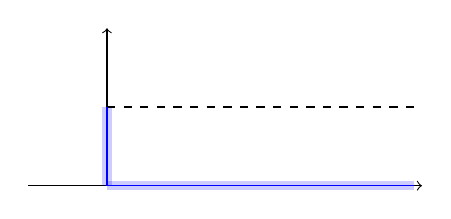
\begin{tikzpicture}
\draw[->] (-1,0) -- (4,0);
\draw[->] (0,1) -- (0,2);
\draw[color=blue] (0,1) -- (0,0);
\fill[opacity = 0.2, blue] (-0.4ex,0) -- (-0.4ex,1) -- (0.4ex,1) -- (0.4ex,0) -- cycle;
\fill[opacity = 0.2, blue] (0,-0.4ex) -- (3.9, -0.4ex) -- (3.9, 0.4ex) -- (0,0.4ex) -- cycle;
\draw[color=blue] (0,0) -- (3.9,0);
\draw[dashed] (0,1) -- (4,1);
\end{tikzpicture}
\caption{Representación gráfica de la unión de $S_1$ y $S_2$}
\end{figure}

\spart

\[\convx{S} = \{x = \sum^{n+1}λ_ix_i\;λ_i \geq 0, \sum λ_i = 1\; x_i\in S\}\]

Tomando \[k = \{(λ_1,λ_2,...,λ_{n+1},x_1,...,x_{n+1}) \;λ_i \geq 0, \sum λ_i = 1\; x_i\in S\}\]

Y construimos: $\appl{f}{k}{\convx{S}}$ tal que $f(λ_1,λ_2,...,λ_{n+1},x_1,...,x_{n+1}) = \sum^{n+1}λ_ix_i$ y esta función es continua.

Tenemos $k$ compacto (por ser $S$ compacto) y que  $f(k) =\convx{S}$, siendo $f$ continua. Entonces, $\convx{S}$ es compacto (por ser imagen continua de un compacto).

\end{problem}

\begin{problem}[9]

Encuentra un ejemplo que muestre que la implicación

\[S_1,S_2 \text{ convexos cerrados} \implies S_1+S_2\text{ es cerrado}\]

no es cierta en general. Prueba que esta implicación es cierta cuando al menos uno de los 2 conjuntos $S_1$ o $S_2$ se supone compacto.

\solution

\[S_1 = \{ (x_1,x_2) \in \real^2\tq\; x_2\geq \rfrac{1}{x_1} \;x_1 > 0\}\]
\[S_2 = \{(x_1,0) \in \real^2\tq x_1\in\real\}\]

Vamos a construir $S_1 + S_2$


\begin{figure}[hbtp]
\centering
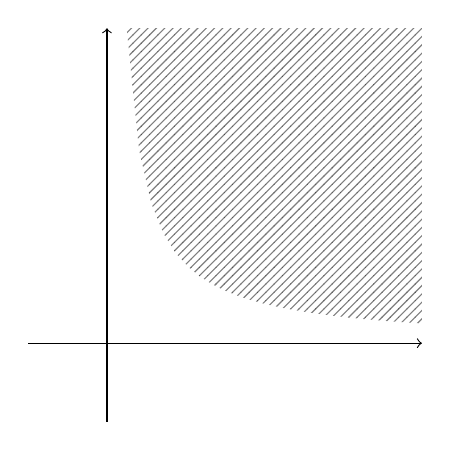
\begin{tikzpicture}
\draw[->] (-1,0) -- (4,0);
\draw[->] (0,-1) -- (0,4);
\fill[opacity = 0.5,black,pattern=north east lines] (4,4) -- plot[variable=\t,samples=25,domain=0.25:4] (\t,1/\t);
\end{tikzpicture}
\caption{Representación gráfica de la suma de $S_1$ y $S_2$}
\end{figure}


\[S_1 + S_2  = \{(x_1,x_2)\tlq x_2>0\}\]

\[(0,0) = \lim (\underbrace{x_k}_{\in S_1} + \underbrace{y_k}_{S_2})\]

Para que sea la suma sea cerrada, necesitaríamos $\{y_k\},\{x_k\} \to (0,0)$ y en este caso no es así. Vamos a ver que con que uno de los 2 conjuntos sea acotado, la suma ya es acotada.

\begin{prop}

$S_1,S_2$ convexos y cerrados, con $S_1$ acotado.

Tomamos $x_k + y_k \in S_1 + S_2$ y tenemos $\lim(x_k + y_k) = z$.

Entonces,
\[z\in S_1 + S_2\]
\end{prop}
\begin{proof}
Existe una subsucesión convergente $\{x_{k_i}\}$de $\{x_k\}$, por ser $S_1$ compacto.
Sea $\gor{x} = \lim x_{k_i}$, con $\gor{x}\in S_1$.

La correspondiente subsucesión de $y_k$ también converge (ya que sino la suma no puede converger)

\end{proof}

\end{problem}

\begin{problem}[10]

$S$ convexo es la intersección de todos los subespacios cerrados que lo contienen.

Formalmente:

\[S = \bigcap_{\begin{array}{c}S\subset H_i\\H_i\text{ compacto}\end{array}} H_i\]

\solution

$S\in \bigcap$ es trivial. 

\[\left.\begin{array}{c} x\in\bigcap H_i\\x\not\in S \end{array}\right\} \implies \exists p≠0, α\in\real p^ty\leq α ∀y\in S p^t x >α\]


\end{problem}

\begin{problem}[11]

Sean $S_1,S_2$ dos conjuntos convexos no vacíos de $\real^n$ tales que $S_1\cap S_2 = \emptyset$. 
Demuestra que existe $p ∈ \real^n , p≠0$, tal que

\[\inf\{p^Tx: x\in S_1\} \geq \sup\{p^Tx : x\in S_2\}\]

Si además, los conjuntos son cerrados y uno de ellos es acotado, demostrar que existe $\rho \in \real^n,\rho ≠ 0, ε > 0$ tales que 

\[\inf\{p^Tx: x\in S_1\} \geq ε + \sup\{p^Tx : x\in S_2\}\]

\textit{Sugerencia: Para la primera parte, considera $S = \{x_1 - x_2 : x_1 \in S_1, x_2 \in S_2\}$ y aplica algún teorema de separación}

\solution


\[ S = \{x_1-x_2 \tq x_1\in S_1, x_2\in S\]

Es convexo, y tenemos $S_1\cap S_2 = 0 \implies 0\not\in S$.

Por ser $\gor{S}$ cerrado y convexo, tenemos 2 posibilidades $0\in S$ o $0\not\in S$:
\[0\not\in \gor{S}\implies \exists p≠0, \exists α\in ℝ p^tx\geq α>0 ∀x\in S\]

\[
\implies p^tx_1 \geq α + p^tx_2 ∀x_i\in S_i
\]


Si por el contrario:

\[
0\in \gor{S} - S \implies 0 \in \partial S \implies \exists p≠0, p^tx\geq 0, ∀x\in S
\]

Eso último se debe a $p^tx_1 ≥ p^tx_2, ∀x_i\in S_i$



\end{problem}

\begin{problem}[12]

\solution

\begin{defn}[Función\IS soporte]
\[S_c(p) = \sup\{p^tx\;:x\in C\}\]
La utilidad de la función soporte es poder comparar funciones en vez de trabajar con conjuntos. Esto está muy bien porque en general es más fácil trabajar con funciones que con conjuntos sobretodo en temas de convergencia.
\end{defn}



Queremos probar que:

\[C = D \dimplies S_C(p) = S_D(p)\]

$\implies)$: Trivial

$\impliedby)$: Supongamos que existe $\gor{x}\in D \tlq \gor{x}\notin C$. De esta manera, podemos aplicar un teorema de separación, es decir:

\[∃p≠0 \tlq p^tx≤α ∀x∃C \implies S_C(p) ≤α \wedge S_D(p) > α \]


\end{problem}

\begin{problem}[13]
Demuestra que si $x$ es una solución factible básica de $S = \{x : Ax = b, x ≥ 0\}$, entonces
es un punto extremo de S.

\solution

$x$ es una solución factible básica si al elegir una base, tenemos: \[x = \begin{pmatrix}B^{-1}b\\0\end{pmatrix} \equiv \begin{pmatrix}\gor{b}\\0\end{pmatrix}\]

Vamos a escribir $x$ como combinación convexa de puntos y ver que esos puntos son iguales a $x$, es decir:

\[\begin{pmatrix}B^{-1}b\\0\end{pmatrix} = λx_1 + (1-λ)x_2 = λ\begin{pmatrix}X_{1B}\\X_{1N}\end{pmatrix} + (1-λ)\begin{pmatrix}X_{2B}\\X_{2N}\end{pmatrix}\]

Como $x_1≥0,x_2≥0 \implies X_{1N} = X_{1B} = 0$. Entonces, tenemos para $i=1,2$:

\[x_i = \begin{pmatrix}X_{iB}\\0\end{pmatrix} \implies Bx_{iB} + N0 = b \implies x_{iB}B^{-1}b = \gor{b}\]


\end{problem}


\begin{problem}[14]
Halla los puntos extremos de los siguientes conjuntos:

\ppart $S = \{(x_1,x_2) \in \real^2 : x_1 + 2x_2 \geq 2, -x_1+x_2 = 4, x_1,x_2\geq 0\}$
\ppart $S = \{(x_1,x_2,x_3) \in \real^3 : x_1 + x_2 + x_3 \leq 10, -x_1+2x_2 = 4, x_1,x_2,x_3\geq 0\}$

\solution

\spart 
\label{ej:ejercicio2.14.a}
Aunque el problema se puede resolver sólo gráficamente, vamos a solucionarlo también algebraicamente.


\begin{figure}[hbtp]
\centering
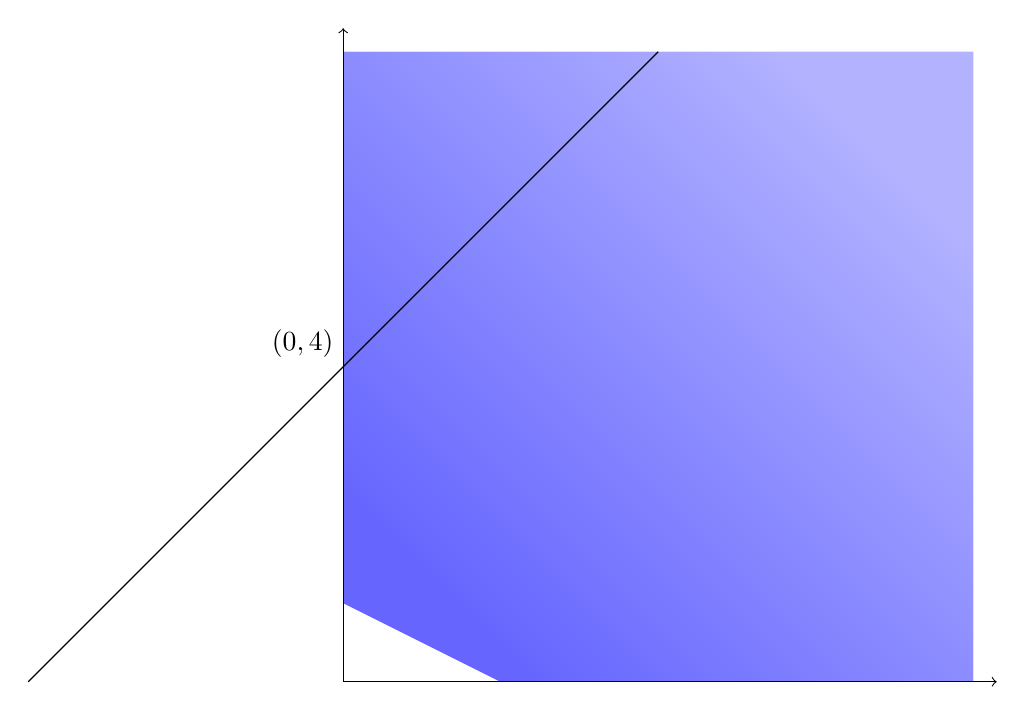
\begin{tikzpicture}
\fill[shading = axis,rectangle, left color=blue!60!white, right color=blue!30!white,shading angle=135,blue!60!white] (0,1) -- (2,0) -- (8,0) -- (8,8) -- (0,8);
\node[anchor=south east] at (0,4) {$(0,4)$};
\draw (-4,0) -- (0,4) -- (4,8);
\draw[->] (0,0) -- (0,8.3);
\draw[->] (0,0) -- (8.3,0);
\end{tikzpicture}
\caption{Solución gráfica del \fref{ej:ejercicio2.14.a}}
\end{figure}

Para resolverlo algebraicamente, tenemos que ir probando con las bases hasta obtener $\gor{b} ≥ 0$. Lo primero que hay que hacer es reconstruir con las variables de holgura, es decir:

\[S = \{(x_1,x_2) \in \real^2 : x_1 + 2x_2 - x_3 = 2, -x_1+x_2 = 4, x_1,x_2,x_3\geq 0\}\]


La solución es:

\[
B = \begin{pmatrix}2&-1\\1&0\end{pmatrix} \implies \gor{b} = \begin{pmatrix}4\\6\end{pmatrix} ≥ \begin{pmatrix}0\\0\end{pmatrix}
\]

\spart 

\todoby{Uceda}

\begin{figure}[hbtp]
\centering
\begin{tikzpicture}
\draw[->] (0,0,0) -- (0,0,4);
\draw[->] (0,0,0) -- (0,4,0);
\draw[->] (0,0,0) -- (4,0,0);
\end{tikzpicture}
\end{figure}
\end{problem}


\section{Hoja 3}

\begin{problem}[1]

Resolver utilizando el algoritmo de simplex el problema:

\begin{ioprob}
\goal{$x_2 - 3x_3 + 2x_5$}
\restrictions{$x_1+3x_2-x_3+2x_5 = 7$}{$-2x_2 + 4x_3 + x_4 = 12$}{$-4x_2 + 3x_3 + 8x_5 + x_6 = 10$}{$x_i \geq 0$}{}
\end{ioprob}

\solution

Vamos a construir la tabla del simplex:


\begin{table}[hbtp]
\centering
\begin{tabular}{c|cccccc}
$c_j$&0&1&-3&0&2&0\\\hline
Variables & $x_1$&$x_2$&$x_3$&$x_4$&$x_5$&$x_6$\\\hline
7&1&3&-1&0&2&0\\
12&0&-2&\textcolor{red}{4}&1&0&0\\
10&0&-4&3&0&8&1\\\hline
$z_j - c_j$ & 0&-1&3&0&-2&0
\end{tabular}
\end{table}

Incluimos la solución final, para terminar el problema en casa. Tras 2 iteraciones obtenemos:


\begin{table}[hbtp]
\centering
\begin{tabular}{c|cccccc}
\hline
4&$\rfrac{2}{5}$&1&0&0.1&0.8&0\\
5&0.2&1&0.3&0.4&0\\
11&1&0&0&-0.5&10&1\\\hline
&-0.2&0&0&-0.8&$-\rfrac{12}{5}$&0
\end{tabular}
\end{table}

Entonces, la solución sería:

\[
\gor{x} = (0,4,5,0,0,11)
\]
\end{problem}

\begin{problem}

\solution
\todoby{Uceda}
\end{problem}

\begin{problem}[3]

\solution

Lo primero es escribir el problema en forma estándar:


\begin{ioprob}
\goal{$\min \sum_{i=1}^3 c_ix_i$}
\restrictions{$x_1-x_2+5x_3 + x_4 = 10$}{$2x_1 - x_2 + x_3 + x_4 = 40$}{$x_i \geq 0$}{}{}
\end{ioprob}

\spart 

Cogemos una base y operamos:

\[B = \begin{pmatrix}1&0\\0&1\end{pmatrix} \to B^{-1}b = b = \begin{pmatrix}10\\40\end{pmatrix}\geq \begin{pmatrix}0\\0\end{pmatrix} \to (0,0,0,10,40)\]

Como $B^{-1}b \geq 0$, $(0,0,0,10,40)$ es un punto extremo.

Tomando por ejemplo:

\[B = \begin{pmatrix}5&0\\3&1\end{pmatrix} \to ... \to (0,0,2,0,34)\]
 
Obtenemos otro punto extremo.

\textbf{Dirección extrema} 

\[
B= 
	\begin{pmatrix}
	1&0\\
	0&1
	\end{pmatrix}\;\; 
a_j = a_2\implies B^{-1}a_2 = 
\begin{pmatrix}
-1\\
-1
\end{pmatrix}\geq 
\begin{pmatrix}
0\\
0
\end{pmatrix} \to d = α
\begin{pmatrix}
0\\
1\\
0\\
\hline 1\\1
\end{pmatrix}\]

\spart

Para cualquier $c_1,c_3$, mientras tomemos $c_2$ negativo no vamos a tener nunca una solución óptima. 

\spart 

Para tener infinitas soluciones óptimas, necesitamos vectores de coeficientes distintos que nos den el mismo valor objetivo.

Podemos tomar $c_1,c_2,c_3$ de tal manera que los 2 puntos extremos que tenemos calculados antes tengan el mismo valor objetivo. De esta manera,  el segmento que une los 2 puntos tiene el mismo valor objetivo. 
\end{problem}


\begin{problem}[4]

Dado un problema de optimización lineal $\min c^\top x$, sujeto a $Ax = b, x ≥ 0$, ¿es posible conseguir un
problema en el que no exista solución óptima finita cambiando únicamente el vector b? Responde a
la misma pregunta para el vector c

\solution

Los teoremas de caracterización nos daban una condición de existencia de solución en caso de cosas en las que no influye $b$, por lo que $b$ no influye y por lo tanto no es posible conseguirlo.

En cuanto al $c$, simplemente con cambiarlo de signo se revienta todo.

\end{problem}

\begin{problem}[5]

\ppart Supongamos que $S≠Ø$ y que para un cierto vector no nulo d ≥ 0, $d∈\real^n$ , se verifica $Ad = 0$ ¿Puede asegurarse entonces que existe un vector $c≠0$ tal que el problema tiene solución
óptima no acotada?

\ppart ¿Puede ocurrir que una solución óptima tenga más de m componentes estrictamente positivas?

\ppart Si $\gor{x}\in S$ tiene exactamente m componentes estrictamente positivas, ¿puede asegurarse que $\gor{x}$ es un punto extremo de S?



\solution

\spart 
Como $S≠Ø$, tenemos $\gor{x}\in S$ y tal que $\gor{x} + λd\in S ∀λ>0$.

Esto quiere decir que hay una dirección extrema, en la que a lo largo de ella, nunca salimos del conjunto factible.
Podemos tomar cualquier $c$ tal que $c^\top d<0$, por ejemplo $c=-d$

\spart Sí puede ocurrir

\spart Sabemos que punto extremo $\dimplies$ solución factible básica. No puede asegurarse, ya que podemos fijar $n-m$ coordenadas iguales a $0$. Si las otras $m$ no forman una base, no podemos despejar para tener un punto extremo. Por ejemplo:


\begin{ioprob}
\goal{}
\restrictions{$x_1+x_3+x_4 = 1$}{$x_2+x_3+x_4=1$}{$x_i≥0$}{}{}{}
\end{ioprob}

En este problema tenemos $n=4$ y $m=2$. El punto $p = \left(0,0,\rfrac{1}{2},\rfrac{1}{2}\right)$ tiene exactamente 2 coordenadas positivas. No es una $SFB$ por lo que no es un punto extremo.

No es una $SFB$ porque $a_3 = a_4 = \begin{pmatrix}1\\1\end{pmatrix}$, por lo que $\{a_3,a_4\}$ no forman una base.

\end{problem}


\begin{problem}[6]

\ppart Calcula la matriz $A$ y el vector $b$.

\ppart Supongamos que el vector de costes $c = (1, 3, 1, 0, 0)$ se reemplaza por $c^\top = c + λγ$, siendo λ un número no negativo e $γ = (1, 1, 1, 0, 0)$. ¿Para qué valores de λ sigue siendo solución óptima $x = (12, 0, 0, 0, 16)$ ?

\solution

\spart 

Cada columna $y_j = B^{-1}a_j$. Si conociéramos $B^{-1}$, ya tendríamos todo. Vamos a descubrir $B$.

\[
	\left.\begin{array}{c}
		y_4 = B^{-1}\begin{pmatrix}1\\0\end{pmatrix} = \begin{pmatrix}1\\1\end{pmatrix}\\
		y_5 = B^{-1}\begin{pmatrix}0\\1\end{pmatrix} = \begin{pmatrix}0\\1\end{pmatrix}
	\end{array}\right\} \implies B^{-1} = \begin{pmatrix}1&0\\1&1\end{pmatrix} \implies B = \begin{pmatrix}1&0\\-1&1\end{pmatrix}
\]

Ahora podemos calcular:

\[
	a_j = By_j \implies 
	\left\{ 
		\begin{array}{c}
			a_2 = \begin{pmatrix}4\\2\end{pmatrix}\\
			a_3 = \begin{pmatrix}3\\-1\end{pmatrix}\\
		\end{array}
	\right.
\]

Con esto:

\[
	A = 
		\begin{pmatrix}
			1&4&3&1&0\\
			-1&2&-1&0&1
		\end{pmatrix}
\]

\textbf{Otra posibilidad} 

\[
	\begin{pmatrix} 1&4&3&1&0 \\ 0&6&2&1&1 \end{pmatrix} \overset{Gauss}{\to} \left(\begin{array}{c|c} Λ \begin{array}{cc}1&0\\0&1\end{array}\end{array}\right) = A
\]

\spart Su ek problema es de maximización, la tabla es óptima si $z_j - c_j ≥ 0 ∀j∈ℕ$.

El caso general, para un $\gamma$ dado sería:

\begin{align*}
	\hat{z_j} - \hat{c_j} = \hat{c}^\top y_j - \hat{c}_j &= (c^t_B + λ\gamma_B)'y_j - (c_j + λ\gamma_j) = (c_B^\top y_j - c_j) + λ(\gamma^\top_By_j - \gamma_B) =
\end{align*}
\begin{align*}
	 \underbrace{(z_j - c_j)}_{≥0} + λ(\gamma_By_j - γ_j) &\overset{?}{≥} 0 ∀j∈ℕ
\end{align*}

Mientras se mantenga la desigualdad, tendremos solución óptima. 

Si $∀j∈ℕ$, entonces la desigualdad se mantiene ya que $(\gamma_By_j - γ_j) ≥ 0 $. Además, se mantiene $∀λ$.

Si $∃j∈ℕ\tq γ_b^\top y_j - γ_j < 0$, entonces $λ$ no puede tomar cualquier valor positivo. Como máximo, $λ = \min\{\text{algo}\}$. ¿Cuánto podemos aumentar $λ$? 

\[λ ≤ \min\left\{  \frac{z_j - c_j}{-(γ_B^\top y_j - γ_j)} \right\}\]

Para este caso concreto (en el que estamos maximizando y no minimizando, con lo que hay un signo que no cambiamos)

\[
	γ_B = (1,0)' \to
	(1,0)y_j - γ_j = 
	\begin{pmatrix}
		4-1 = 1\\
		3-1 = 2\\
		1-0 = 1
	\end{pmatrix}
\]


\end{problem}


\begin{problem}[7]

Este es un problema de examen (ligeramente cambiado)


\solution

\begin{table}
\centering
\begin{tabular}

\end{tabular}
\end{table}

a≥0 (está en la pizarra pero no se de donde sale)-

\spart 

En este caso, $z_j - c_j = -c_j$, si $a_j∈B$

Por otro lado:
\[ z_2 - c_2 = -b ≤ 0 \implies b≥0\]
\[ z_3 - c_3 = -e ≤ 0 \implies e≥0\]

\spart $b<0$ para que mejore al aumentar y $c,d≤0$ para que podamos aumentar todo lo que queramos. 

\textbf{¿Y si $b=0$?}

\spart $b,e≥0$ para que sea óptima y para tener una dirección extrema, necesitamos $c,d≤0$.

\end{problem}
\printindex
\end{document}
